% !TeX spellcheck = en_US

\documentclass[a4paper,14pt]{extreport}

\usepackage{enumitem}
\usepackage{docdef}

\addbibresource{../bibliography/sources.bib}

\begin{document}
	\maketitle
	

	\clearpage
	
	% Название содержания меняем
	\renewcommand{\contentsname}{Содержание}
	\tableofcontents
	
	\clearpage
	
	\bsuabstract
	{
		This paper examines methods for extraction of economic cycles, identification of their turning points, and prediction of future values. This paper also compares the results of these methods when used to identify cycles in the GDP of the Republic of Belarus. Methods reviewed: double Hodrick-Prescott filtering, Hamilton's proposed method,  Markov-switching autoregressive models (MS-ARX), and SARIMAX models. The work also includes a short description of the development of a Python-language library for time series analysis and modelling, which includes implementations of the above models.
		
	}{
		В данной работе рассматриваются методы выделения экономических циклов, определения их поворотных точек, и предсказания будущих значений. Также сравниваются результаты применения этих методов при идентификации циклов в ВВП Республики Беларусь. Рассмотренные методы: двойное использование фильтра Ходрика -- Прескотта, метод Хамильтона, авторегрессионные модели с Марковским переключением состояний (MS-ARX), модели SARIMAX. В работе также приводится краткое описание разрабатываемой библиотеки программ на языке Python, предназдаченной для анализа и моделирования временных рядов. Библиотека включает разделы, посвященные вышеописанным моделям.
	}
	
	\clearpage
	{
		\centering\normalfont\Large\bfseries{Обозначения и сокращения} \par
		\nopagebreak % чтобы не оторвать заголовок от текста
	}

	\textbf{ВВП / GDP} -- валовой внутренний продукт (Gross Domestic Product);
	
	\textbf{ИЭН / ESI} -- индекс экономических настроений (Economic Sentiment Index);
	
	\textbf{ОЭСР / OECD} -- Организация экономического сотрудничества и развития (Organization for Economic Cooperation and Development);
	
	\textbf{НБЭИ / NBER} -- Национальное бюро экономических исследований США (National Bureau of Economic Research)
	
	\textbf{X13-ARIMA-SEATS} и \textbf{TRAMO/SEATS} -- методы сезонной корректировки временных рядов;
	
	\textbf{MS-ARX} -- модель авторегрессии с Марковским переключением состояний и экзогенными переменными (Markov-Switching AutoRegression with Exogenous variables);
	
	\textbf{SARIMAX} -- сезонная, интегрированная модель авторегрессии и скользящего среднего с экзогенными переменными (Seasonal AutoRegressive Integrated Moving Average model with Exogenous variables).
	
	\clearpage
	
	
	\chapter*{Введение}
	\addcontentsline{toc}{chapter}{Введение}
	\markboth{Введение}{Введение}
	В работе представляются результаты, полученные автором при решении задач связанных с выделением циклических компонент макроэкономических рядов статистическими фильтрами, а также связанных с построением и применением моделей с марковскими переключениями состояний (из семейства MS-VARX) и сезонной ARIMA-модели (SARIMAX).	В качестве исходных данных использующиются ВВП Республики Беларусь и индекс экономических настроений (ИЭН) белорусской экономики (полученный на основе опросных данных системы мониторинга Национального банка Республики Беларусь). 
		
	Исследования в данном направлении проводились в Белорусском государственном университете в 2016-2017 гг. в рамках НИР "Разработка системы опережающих экономических индикаторов и экономических диффузных индексов для основных видов экономической деятельности и экономики Республики Беларусь в целом с использованием экономико-математических, эконометрических методов и моделей на основе данных системы мониторинга предприятий Национального банка Республики Беларусь". Модельный и программный инструментарий для построения указанных  индексов и их применения в предиктивных эконометрических моделях для реального ВВП, а также в моделях с марковскими переключениями состояний для анализа бизнес-цикла белорусской экономики представлены в заключительном отчете о НИР \cite{esiMaking}.
	
	\bigskip
	%\section
	\textbf{Теория экономических циклов}
	
	В рамках концепции экономического цикла, используемой в НБЭИ (Национальное бюро экономических исследований) США, подразумевается последовательная смена двух фаз базового экономического индикатора, называемых периодами <<роста>> (growth)  и <<спада>> (recessions) экономической активности. При этом поворотные точки соответствуют <<пику>> (максимальной точке роста) и <<дну>> (минимальной точке спада) экономического цикла \cite{nberDevelopment}.  В рамках концепции ОЭСР (Организации экономического сотрудничества и развития) допускается  детализация основных фаз цикла относительно долгосрочного тренда с выделением периодов <<роста>> и <<замедления>> (выше линии тренда), а также  -- <<спада>> и <<восстановления>>  (ниже линии тренда) \cite{oecdCycleExtraction}. Поворотные точки в данном случае соответствуют моментам начала замедления роста и начала восстановления после спада. 
	
	Одной из ключевых задач анализа и прогнозирования экономической активности является разработка систем раннего обнаружения смены фаз экономических циклов на основе специально разработанных экономических индикаторов. Для получения ранних сигналов о смене фаз и оценивания моментов смены фаз, называемых поворотными точками, в рамках указанных систем применяются так называемые опережающие экономические индикаторы (leading economic indicators) \cite{oecdCLI}. В рамках \cite{esiMaking,esiMakingAlt,esiExtra} была разработана система опережающих индикаторов для Республики Беларусь, в том числе Индекс Экономических Настроений/Economic Sentiment Indicator (ИЭН/ESI). В настоящей работе в качестве опережающего и базового экономических индикаторов используются соответственно временные ряды значений индекса экономических настроений и реального ВВП Республики Беларусь в ценах 2014 г., в месячном исчислении с мая 2005 г. по январь 2017 г., полученные в рамках указанной НИР.
	
	\bigskip
	%\section
	\textbf{Методы выделения циклической составляющей}
	
	Для периодизации экономических циклов необходимо выделить из временных рядов реального ВВП и ИЭН циклические составляющие, на основании которых затем оцениваются поворотные точки циклов. На опережающий характер ИЭН указывает тот факт, что поворотные точки его цикла предшествуют поворотным точкам цикла реального ВВП. В настоящее время, основным методом выделения догосрочной циклической состовляющей являются статистические фильтры. Наиболее популярным является фильтр Ходрика -- Прескотта \cite{oecdCycleExtraction,estrellaFilterDo}. Данный фильтр используется в указанной выше НИР, а так же в рамках данной работы. 
	
	В недавней статье Дж. Хамильтона \cite{hamHP} указывается на проблемы, возникающие при использовании фильтра Ходрика -- Прескотта, и предлагается свой метод выделения долгосрочного цикла. Этот метод, так называемый <<фильтр Хамильтона>>, также подвергается некоторой критике.
	
	В проводимом исследовании используются оба метода, т.е. основанные на фильтрах Ходрика -- Прескотта и Хамильтона, для выделения долгосрочного цикла, и проводится сравнительный анализ поворотных точек циклов, получаемых с помощью данных фильтров, а так же экспертным путем. Подобное исследование ранее не проводилось на белорусских данных. Полученные в рамках данной работы результаты являются новыми, и частично опубликованы в [A4].
	
	\bigskip
	%\section
	\textbf{Методы оценивания поворотных точек}
	
	Для оценки поворотных точек существуют несколько широко используемых методов. Один из самых популярных -- алгоритм Брай -- Бошана \cite{bryCyclicalAnalysis}, который состоит из несколько этапов (с минимальной длительностью цикла в 15 месяцев и отдельных фаз в 5 месяцев). Другой популярный метод -- модели с переключающимися режимами, впервые популяризированый работой Хамильтона \cite{hamNewApproach}. Результаты Хамильтона с MS-AR для бизнес--цикла США во многом сходились с периодизацией NBER. Многие научные исследования \cite{bodmanCanada,brunoItaly,hardingTwoMethods} указывают на сопоставимость Марковских моделей и традиционных методов, однако на практике они редко используется из--за сравнительной трудоемкости и непрозрачности. Существуют и другие подходы, которые так же не используются из--за сравнительной сложности вычислений.
	
	В данной работе используюся оба подхода для решения указанной задачи.
	
	
	
	\chapter{Эконометрические модели и методы анализа циклических изменений в экономике}
	
	
	\section{Использование статистических фильтров для выделения трендов и циклов из экономических временных рядов}
	
	Статистический фильтр Ходрика -- Прескотта \cite{hp_orig_paper} широко используется в различных эконометрических исследованиях, связанных с выделением долгосрочных трендов и циклов из экономических временных рядов. Выделение трендовой компоненты исследуемого временного ряда является важным этапом при решении такой задачи макроэкономического анализа, как определение потенциального выпуска и разрыва выпуска (кредитного разрыва) в рамках формирования денежно-кредитной политики центральными банками \cite{zubarev_gap, demidenko_gap, schuler_detrend}. При этом трендовая компонента временного ряда рассматривается как потенциальный выпуск или равновесный реальный ВВП, а остаточная составляющая временного ряда, включающая циклический и шумовой компонент,  соответствует отклонениям его фактических значений  от ожидаемых в равновесном состоянии и интерпретируется как разрыв выпуска. В рассматриваемом контексте важной является задача прогнозирования значений потенциального выпуска и разрыва выпуска в экономике на ближайшую перспективу. 
	
	Фильтр Ходрика -- Прескотта в настоящее время также является рекомендуемым методом выделения долгосрочных циклов в рамках методологии ОЭСР \cite{oecdCLI, oecdCycleExtraction}, используемой для анализа бизнес-циклов на основе опережающих экономических индикаторов. В контексте подобного исследования он применялся для выделения циклических компонент из временных рядов реального ВВП и индекса экономических настроений (ИЭН) белорусской экономики \cite{esiMakingAlt}. 
	
	Однако, широко используемый стандартный одномерный фильтр Ходрика -- Прескотта обладает рядом общеизвестных недостатков.  К ним относятся: 
	
	\begin{itemize}
		\item смещение оценок значений тренда в начальных и конечных точках временного ряда (<<end-point bias problem>>) и высокая чувствительность этих оценок к добавлению новых наблюдений; 
		\item отсутствие строгой формализации правила выбора для значения параметра фильтра (<<параметра $\lambda$>>), определяющего степень гладкости тренда и критическим образом влияющего на свойства выделяемых компонентов временного ряда.
	\end{itemize}
	
	Заметим, что смещение имеет место и в начальных точках временного ряда, но оно не является критичным в контексте задачи прогнозирования.
	
	Также имеют место особенности применения данного фильтра к временным рядам, в зависимости от того, содержат ли они детерминированные или стохастические тренды \cite{kharin8}. Это можно объяснить тем, что в основе процедуры выделения тренда лежит компромисс между степенью гладкости получаемого детерминированного тренда и его близости к фактическим данным. При этом ожидается, что остаточная составляющая представляет собой комбинацию цикла и шумового компонента, который является стационарным временным рядом и имеет нулевое среднее значение. Можно предположить, что указанные свойства трендовой и остаточной составляющих достижимы, если сглаживаемый временной ряд относится к классу нестационарных временных рядов с детерминированными трендами (trend stationary -- TS-моделей).  В противном случае, если временной ряд содержит стохастический тренд, т. е. относится к классу DS-моделей (difference stationary), следует ожидать нестационарность шумового компонента в остаточной составляющей, следствием которой являются ложные циклы (spurious cycles) и ложные корреляции (spurious correlations). Эти недостатки отмечаются исследователями при обработке большей части макроэкономических и финансовых временных рядов \cite{schuler_detrend, harvey_detrend, pederson_hp}, проявляющих свойства процессов случайного блуждания.
	
	В этом контексте Дж. Хамильтон выступил с критикой использования фильтра Ходрика -- Прескотта в качестве универсального подхода к выделению долгосрочных трендов. В своей рабочей статье он приводит аналитическое обоснование следующих недостатков фильтра \cite{hamHP}:
	
	\begin{enumerate}
		\item фильтр индуцирует ложные циклы, когда применяется к временным рядам с высоким порядком интегрирования и содержащим стохастический тренд;
		\item конечные значения тренда, выделяемого из временного ряда, существенно отличаются от срединных значений и описывают ложную динамику;
		\item статистическая формализация проблемы выбора параметра сглаживания тренда обычно приводит к значениям параметра, который в значительной степени противоречит обычной практике.
	\end{enumerate}
	
	В этой же статье автором предлагается альтернативный метод выделения тренда, получивший в литературе название <<регрессионный фильтр Хамильтона>> (Hamilton's regression filter). К настоящему моменту известен ряд публикаций, посвященных сравнительному анализу фильтров Ходрика -- Прескотта и Хамильтона в практических исследованиях. В рабочей статье \cite{schuler_detrend} проведен сравнительный анализ обоих фильтров при анализе <<кредитного разрыва>> в экономике (credit-to-GDP gap) на основе квартальных временных рядов США. В работе \cite{haubrich_cyc_bank} при анализе цикличности банковского капитала использовались оба фильтра и в целом получены схожие результаты.
	
	Фильтр Хамильтона, в отличие от фильтра Ходрика -- Прескотта, еще не использовался белорусскими исследователями. Поэтому представляется актуальным сравнительный анализ обоих фильтров при обработке белорусских макроэкономических временных рядов, обладающих такими особенностями, как короткая длина и частые структурные изменения. Данная статья посвящена сравнительному анализу результатов применения фильтров для выделения трендовый и циклических компонентов временных рядов при решении задачи анализа бизнес-цикла белорусской экономики в рамках методологии ОЭСР \cite{oecdCycleExtraction, esiMaking}. 
	
	\section{Общее описание используемых статистических фильтров}
	
	\subsection{Фильтр Ходрика -- Прескотта}
	
	При использовании данного фильтра априорно предполагается, что временной ряд   имеет структуру, допускающую его нестационарность в виде наличия тренда, а также присутствие циклических изменений. Таким образом, общая структура временного ряда допускает представление:
	
	\begin{equation}
	y_t = \tau_t + c_t + \varepsilon_t, \quad t \in \overline{1,T},
	\label{eq:decomposition}
	\end{equation}
	
	где временные ряды  $\tau_t$, $c_t$ и $\varepsilon_t$ соответствуют трендовой, циклической и случайной шумовой компонентам. 
	
	Обычно выделению тренда предшествует сезонная корректировка временного ряда. Для этой цели могут применяться известные процедуры Census X13, TRAMO-SEATS и др. \cite{oecdCycleExtraction, esiMakingAlt}. 
	
	Фильтр Ходрика -- Прескотта при однократном применении осуществляет декомпозицию временного ряда $y_t$ на тренд $\tau_t$ и остаточную составляющую $\nu_t$ вида
	
	\begin{equation}
	y_t = \tau_t + \nu_t .
	\label{eq:decomp1}
	\end{equation}
	
	Остаточная составляющая включает цикл, искаженный случайным шумом, т. е. 
	
	\begin{equation}
	\nu_t = c_t + \varepsilon_t .
	\label{eq:decomp2}
	\end{equation}
	
	Для выделения тренда $\tau_t$ решается задача оптимизации \cite{hp_orig_paper}: 
	
	
	
	\begin{equation}	
	{
		\min_{ \tau_t }{
			( 
			\sum_{t=1}^{T} (y_t-\tau_t)^2 + 
			\lambda \sum_{t=2}^{T-1} (\tau_{t+1} - 2\tau_t + \tau_{t-1})^2
			)
		}, \quad
		\lambda > 0, 
	}
	\label{eq:hpmineq}
	\end{equation}
	
	где $\lambda > 0$ -- параметр сглаживания тренда: при $\lambda \rightarrow 0$ значения тренда близки к значениям исходного ряда, т. е. $\tau_t \rightarrow y_t$, а при $\lambda \rightarrow \infty$ вид тренда приближается к линейной по времени $t$ функции.
	
	Первое слагаемое в уравнении (\ref{eq:hpmineq}) отвечает за точность подгонки, а второе -- за степень гладкости тренда. Как отмечалось выше, возникает проблема выбора значения параметра   для конкретных условий решаемой задачи. На практике рекомендуются следующие статистически обоснованные значения параметра   в зависимости от интервала наблюдения значений временного ряда: 14400 -- для месячных, 1600 -- для квартальных и 100 -- для годовых временных рядов \cite{hp_orig_paper}. Однако, на практике значения   корректируются с учетом особенностей решаемой задачи, длины предполагаемых циклов и используемых временных рядов. 
	
	Так, например, при анализе «кредитного разрыва» в экономике (credit-to-GDP gap) на основе квартальных временных рядов достаточно большой длины в соответствии с рекомендациями Базель-3 следует полагать $\lambda = 400000$  что соответствует существованию циклов длиной 30 лет.  В то время как при $\lambda = 1600$ ожидаемая длина цикла составляет около 7.5 лет \cite{schuler_detrend}.
	
	Фильтр Ходрика -- Прескотта обладает «свойством симметричности», которое проявляется в использовании начальных и конечных значений временного ряда в процессе сглаживания его срединных значений; иными словами, он является двусторонним фильтром. Следствием данного свойства является смещенность начальных и конечных сглаженных значений. В контексте задачи прогнозирования особую важность приобретает проблема смещения конечных значений тренда. Данная проблема в стандартной версии фильтра решается путем предварительной пролонгации временного ряда (например, с помощью прогнозирования на основе модели ARIMA). Таким образом, интересующие пользователя точки будут находиться уже не в конце временного ряда, а искажению подвергнуться эти пролонгированные (прогнозные) значения. Удобным способом продления временного ряда длиной Т на заданную величину Н с его одновременной сезонной корректировкой является применение метода TRAMO/SEATS для расширенного временного интервала длинной Т+H. Такая возможность имеется во многих статистических и эконометрических пакетах, в том числе в программе ESI Analysis (Economic Sentiment Indicator Analysis), разработанной на языке программирования R в рамках научного проекта, выполнявшегося в НИИ ППМИ БГУ по заданию Национального банка Республики Беларусь в 2016-2017 гг. \cite{esiMaking}. Программа ESI Analysis реализует весь комплекс задач, связанных с построением индекса экономических настроений и его применения для анализа бизнес-цикла белорусской экономики и его поворотных точек.  
	
	Для выделения долгосрочного цикла из временного ряда $y_t$ используется процедура, основанная на двухэтапном применении фильтра Ходрика -- Прескотта. Для этой цели к остаточной составляющей $\nu_t$, полученной после выделении тренда из временного ряда $y_t$, применяется фильтр Ходрика -- Прескотта со значением $\lambda$, соответствующим более краткосрочным колебаниям. В рамках данного исследования, при анализе бизнес-цикла в белорусской экономике на основе месячных временных рядов,  используются рекомендуемые в рамках методики ОЭСР значения параметра $\lambda$:  $\lambda = 42131.155$ для первого и $\lambda = 13.93$ для второго этапа процедуры. Этим значениям соответствуют продолжительности «типичного бизнес-цикла» (от 5 до 8-9 лет) и высокочастотных колебаний (6-12 месяцев). На рисунке \ref{fig:different_lambda} представлены оценки циклической составляющей белорусского ВВП с различными величинами параметра $\lambda$ (соответствуют длине цикла 60, 90 и 120 месяцев) \cite{esiMakingAlt}. Отличия в этих оценках циклических составляющих невелики, за исключением конечных значений.  В описываемых ниже экспериментах используется средний по продолжительности цикла вариант, которому соответствуют вышеуказанные значения параметра $\lambda$.
	
	\begin{figure}
		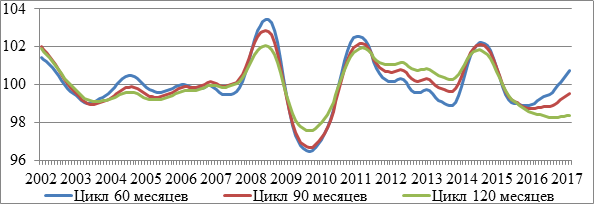
\includegraphics[width=\linewidth]{different_lambdas.png}
		\caption{Оценки бизнес-цикла посредством фильтра Ходрика -- Прескотта в зависимости от предполагаемой продолжительности цикла.}
		\label{fig:different_lambda}
	\end{figure} 	
	
	\subsection{Фильтр Хамильтона}
	
	В фильтре, предложенном Дж. Хамильтоном \cite{hamHP}, долгосрочный тренд в нестационарном временном ряду $y_t$ описывается моделью регрессии, включающей, для момента времени $t+h$, константу и четыре наиболее близких к моменту времени $t$ значения временного ряда: 
	
	\begin{equation}
		y_{t+h} = \beta_0 + \beta_1 y_t + \beta_2 y_{t-1} 
		+ \beta_3 y_{t-2} + \beta_4 y_{t-3} + \nu_{t+h} ,
		\label{eq:ham_filter}
	\end{equation}
	
	где $(h>0)$ -- априорно задаваемый параметр, зависящий от предполагаемой длины цикла. 
	
	При анализе бизнес-цикла по квартальным данным США в \cite{hamHP} предлагается использовать, $h=8$ (для двухгодичных циклов), а в исследованиях кредитных и финансовых циклов $h=20$ (для пятилетних циклов).
	
	Для оценивания параметров модели (\ref{eq:ham_filter}) используется обычный метод наименьших квадратов (МНК). Остаточная составляющая, появляющаяся после подстановки в регрессионное уравнение (\ref{eq:ham_filter}) МНК-оценок параметров $\{\hat{\beta_l}\}, \quad l=\overline{0,4}$, описывается соотношением:
	
	\begin{equation}
		\hat{\nu}_{t+h} = y_{t+h} - \hat{\beta_0} - \hat{\beta_1} y_t 
		- \hat{\beta_2} y_{t-1} - \hat{\beta_3} y_{t-2} - \hat{\beta_4} y_{t-3} .
		\label{eq:ham_resids}
	\end{equation}	
	
	Хамильтоном показано, что для нестационарных интегрированных временных рядов вплоть до порядка $d=4$ остаточная циклическая составляющая $\nu_t$ временного ряда вида (\ref{eq:ham_resids}) включает как циклическую, так и стационарную случайную компоненту, т. е. $\hat{\nu}_{t+h}=c_{t+h} + \varepsilon_{t+h}$. При тех же условиях остаточная составляющая в уравнении (\ref{eq:decomp1}), получаемая с помощью фильтра Ходрика -- Прескотта, может демонстрировать ложные циклы и корреляции. 
	
	Достоинством процедуры Хамильтона является то, что она не использует априорную информацию о конкретном виде модели временного ряда, например о порядке интегрируемости. 
	
	В частном случае, если временной ряд порождается моделью случайного блуждания, т. е. порядок интегрирования ряда равен 1: 
	
	\begin{equation}
		y_t = \beta_0 + y_{t-1} + \varepsilon_t ,
		\label{eq:ham_unitroot}
	\end{equation}
	
	то для МНК-оценок коэффициентов регрессии в уравнении (\ref{eq:ham_resids}) при достаточно большой длине ряда ($T \rightarrow \infty$) значения сходятся к $\beta_1 = 1$ и $\beta_l = 0, l \in \{2, 3, 4\}$ \cite[с. 16-17]{hamHP}. В данном случае исключение тренда по Хамильтону эквивалентно взятию первой разности (со смещением):
	
	\begin{equation}
		\hat{\nu}_{t+h} = y_{t+h} - \hat{\beta_0} + y_{t} .
		\label{eq:ham_unitroot_resid}
	\end{equation}
	
	Для временного ряда с порядком интегрирования 2 при оценке модели (\ref{eq:ham_filter}) следует ожидать получение статистически значимого значения коэффициента регрессии $\hat{\beta_3}$  (для лага -2).  
	
	Указанными свойствами обладают так называемые \textit{разностные фильтры} (difference filters), т.\:е. фильтры, основанные на взятии разностей; следовательно, результаты применения фильтра Хамильтона к временным рядам с невысоким порядком интегрирования могут быть близки к результатам, получаемым с помощью разностных фильтров. В отношении разностных фильтров стоит отметить, что их не следует применять к стационарным временным рядам или временным рядам, содержащим детерминированные тренды из-за возможной генерации ложных циклов \cite{schuler_detrend, harvey_detrend}. Для подобного же утверждения в отношении свойств фильтра Хамильтона для таких рядов требуются дальнейшие исследования. 
	
	В отличие от фильтра Ходрика -- Прескотта, фильтр Хамильтона является «асимметричным» (т. е. односторонним), что позволяет избежать проблемы смещения конечных значений при прогнозировании остаточной составляющей. Так, например, для временного ряда, описываемого моделью случайного блуждания (\ref{eq:ham_unitroot}),  значение остаточной циклической составляющей $\hat{\nu}_{t+h}$ в момент времени $t+h$ формируется на основе известных значений временного ряда $y_{t+h}$ и $y_t$. В общем случае для оценивания тренда и получения остаточной циклической составляющей используется только наблюдаемый временной ряд; это становится особенно важным для коротких временных рядов, а также при наличии структурных изменений в анализируемом временном интервале. Более глубокий сравнительный анализ свойств обоих фильтров проводится в \cite{schuler_detrend}.
	

	
	\section{Модели семейства MS-VARX и их применение для анализа циклических изменений}
	
	\subsection{Общее описание моделей с переключениями состояний}
	Модели с перекюлчением состояний (Regime Switching / $RS$ models) -- это подкласс моделей со структурными изменениями в которых скачкообразно меняются параметры модели. Каждый <<режим>> (класс состояния) в данном случае соответствует отдельному набору параметров, и номер режима $l(t)$ в текущий момент времени $t$ является ненаблюдаемой случайной величиной.
	
	Если номер режима $l = l(t)$ описывается Марковским процессом (текущее состояние зависит только от предыдущего, с матрицей вероятностей перехода), то такую модель называют \textit{марковской моделью переключения состояний} (Markov Switching / MS model). Подробнее эти модели описаны в \cite{malNovopMSVARX}, \cite{mal_methods_nonconstant}.
	
	Модель $MS(L)-VARX(p)$ (Markov--Switching Vector Autoregressive model with exogenous variables) описывается следующим уравнением:
	
	\begin{equation}
		y_{t} = \alpha_{0,l} + \sum_{i=1}^{p} A_{i,l} y_{t-i} + B_{l} x_{t} + \eta_{t}, 
		\quad t = \overline{1,T}
		\label{eq:var_equation}
	\end{equation}
	
	где $L$ -- количество классов состояний, $p$ -- порядок авторегрессии, $x_{t}$ -- экзогенная векторная переменная, $\alpha_{0,l}$ - вектор констант регрессии, и $\eta_{t}$ -- нормально--распределенный белый шум с матрицей $\Sigma_{l}$.
	
	$A_{i,l}, \quad i = \overline{1,p} $ -- авторегрессионные коэффициенты ($A$ -- матрица), $B_{l}$ -- матрица коэффициентов. Эти коэффициенты, как и $\Sigma_{l}$, определены для каждого режима $l$.
	
	$l=l(t) \in \overline{1,L}$ -- номер режима в момент времени $t$, с матрицей вероятности одношаговых переходов для цепи Маркова:
	
	\begin{equation}
		M=
		\left[ {\begin{array}{cccc}
			m_{1,1} & m_{1,2} & ... & m_{1,L} \\
			m_{2,1} & m_{2,2} & ... & m_{2,L} \\
			... & ... & ... & ... \\
			m_{L,1} & m_{L,2} & ... & m_{L,L} \\
			\end{array} } \right]
		, \quad
		\sum_{j=1}^{L} m_{i,j} = 1 \quad \forall i \in \overline{1,L}.
		\label{eq:M_matrix}
	\end{equation}
	
	При $L=2$, можно упростить матрицу:
	
	\begin{equation}
	M=
	\left[ {\begin{array}{cc}
		\sigma_{1} & 1-\sigma_{2} \\
		1-\sigma_{1} & \sigma_{2} \\
		\end{array} } \right].
	\label{eq:M_simplified}
	\end{equation}
	
	Оценивание параметров таких моделей можно проводить с помошью итерационного EM--алгоритма (EM MS--VARX) \cite{malNovopMSVARX} либо методом максимального правдоподобия. Из--за стохастичного характера алгортима сходимость к одному результату не гарантирована.
	
	
	\subsection{Модель MS-ARX}
	
	Если рассматривать одномерные временные ряды, то выделяется подкласс $MS(L)-AR(p)X$:
	
	\begin{equation}  
	y_{t} = \alpha_{0,l} + \sum_{i=1}^{p} \alpha_{i,l} y_{t-i} + \beta_{l} x_{t} + \eta_{t},
	\label{eq:msarx_base}
	\end{equation}
	
	где $\eta_{t}$ -- одномерный гауссовский белый шум с матрицей $\sigma_{l}$. Параметры $\sigma_{l}$, $\alpha_{0,l}$, $\alpha_{i,l}$ и $\beta_{l}$ зависят от режима $l$.
	
	Если рассматривать одномерную экзогенную переменную с лагом $k$, то уравнение модели можно записать:
	
	\begin{equation}  
	y_{t} = \alpha_{0,l} + \sum_{i=1}^{p} \alpha_{i,l} y_{t-i} + \beta_{l} x_{t-k} + \eta_{t}.
	\label{eq:gen-msarx}
	\end{equation}
	
	Обозначим эту модель $MS(L)-AR(p)-X({x}_{-k})$. Оценивание можно проводить по вышеописанными алгоритмами для MS-VARX.
	
	
	\chapter{Экспериментальное исследование эконометрических методов анализа экономических циклов}
	
	\section{Результаты сравнительного анализа фильтров}
	
	\subsection{Выделение тренда и циклической составляющей с шумовым компонентом}
	
	Приведем описание результатов применения фильтров Ходрика -- Прескотта и Хамильтона для решения задачи анализа бизнес-цикла белорусской экономики в рамках методологии ОЭСР \cite{oecdCycleExtraction}. Статистической обработке с помощью указанных фильтров подвергаются два временных ряда, полученные за период наблюдения с мая 2005 г. по январь 2017 г.: 
	
	\begin{enumerate}
		\item базовый экономический индикатор, на основании которого определяется бизнес-цикл белорусской экономики, в виде реального ВВП в ценах 2014 г.;
		\item индекс экономических настроений ИЭН, построенный на основе данных конъюнктурных опросов предприятий в рамках системы мониторинга Национального банка Республики Беларусь.
	\end{enumerate}

	Для обработки временных рядов в настоящем исследовании используется пакет statsmodels языка Python \cite{statsmodels}.
	
	Методология построения и результаты сравнительного анализа циклов данных индикаторов описаны в \cite{esiMakingAlt}. Там же осуществлена оценка поворотных точек для обоих циклов и установлен опережающий характер индекса ESI с периодом опережения в среднем на 4 месяца. Для выделения трендов и циклов из обоих временных рядов в соответствии с методологией ОЭСР \cite{schuler_detrend} использовался фильтр Ходрика -- Прескотта. В связи с появлением нового метода решения данных задач в виде фильтра Хамильтона становится актуальной задача сравнительного анализа результатов, полученных с помощью фильтров Ходрика -- Прескотта и Хамильтона. В данном разделе представляются результаты проведенного сравнения. 
	
	На рисунке \ref{fig:inital_gdp_esi} представлены используемые месячные временные ряды реального ВВП и ИЭН Республики Беларусь. В соответствии с вышеописанными процедурами обработки временных рядов на предварительном этапе осуществлялась сезонная корректировка временных рядов методом X13-ARIMA-SEATS \cite{seasonalManual}.
	
	
	\begin{figure}
		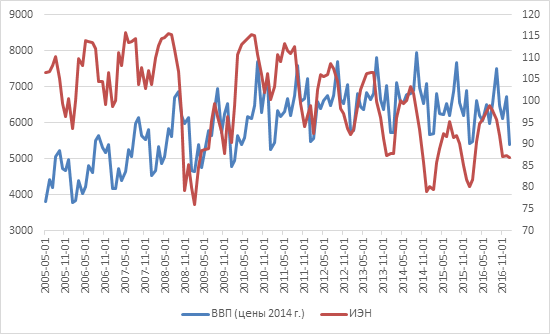
\includegraphics[width=0.8\linewidth]{initial_gdp_esi.png}
		\caption{
			Временные ряды ВВП и ИЭН. 
			Шкала для ВВП -- слева, для ИЭН -- справа. 
		}
		\label{fig:inital_gdp_esi}
	\end{figure} 

	Далее из сезонно скорректированных временных рядов ВВП и ИЭН выделяются трендовые компоненты с применением каждого из фильтров. Параметры сглаживания трендов полагаются следующими: $\lambda=42131.155$ для фильтра Ходрика -- Прескотта \cite{esiMakingAlt} и $h=12$ для фильтра Хамильтона. Данное значение параметра $h$, соответствующее годичному циклу по месячным данным, выбрано в соответствии с общими рекомендациями в рамках фильтра Хамильтона и с учетом относительно короткой длины рассматриваемых временных рядов. Полученные тренды и сезонно скорректированные временные ряды для реального ВВП и ИЭН представлены на рисунках \ref{fig:rr3} и \ref{fig:rr4}.
	
	\begin{figure}
		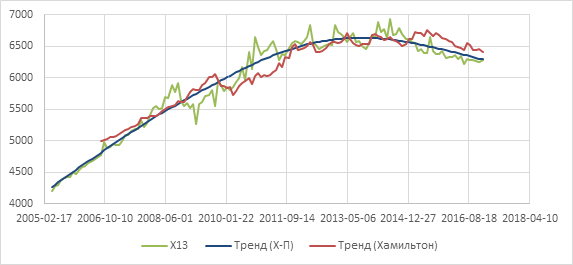
\includegraphics[width=\linewidth]{rr3.png}
		\caption{
			Сезонно скорректированный ряд ВВП и тренды, 
			выделенные фильтрами Ходрика -- Прескотта (Х-П) и Хамильтона. 
		}
		\label{fig:rr3}
	\end{figure}	

	\begin{figure}
		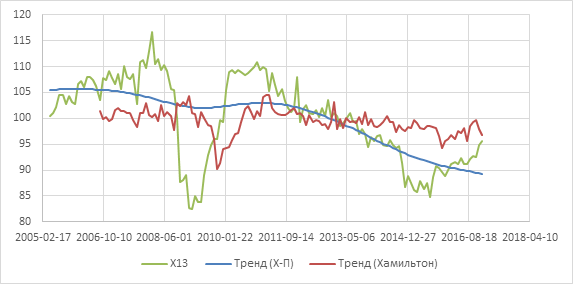
\includegraphics[width=\linewidth]{rr4.png}
		\caption{
			Сезонно скорректированный ряд ИЭН и тренды, 
			выделенные фильтрами Ходрика -- Прескотта (Х-П) и Хамильтона.
		}
		\label{fig:rr4}
	\end{figure}	

	В результате оценивания регрессионных моделей вида (\ref{eq:ham_filter}) получены следующие уравнения трендов для реального ВВП (\ref{eq:ham_fitted1}) и ИЭН (\ref{eq:ham_fitted2}). В квадратных скобках указаны значения t-статистики для теста статистической значимости соответствующих оценок параметров модели, $\hat{\sigma}^2$ представляет собой оценку дисперсии остатков:

	
	\begin{equation}
		y_{t+12} = \underset{[7.63]}{1490.67} 
		+ \underset{[23.21]}{0.918} y_{t}
		- \underset{[-0.43]}{0.017} y_{t-1}
		- \underset{[-2.68]}{0.106} y_{t-2}
		- \underset{[-0.47]}{0.018} y_{t-3}
		+ \hat{\nu}_{t+h}, \quad \hat{\sigma}^2=5851 ,
		\label{eq:ham_fitted1}
	\end{equation}
	
	\begin{equation}
		y_{t+12} = \underset{[7.01]}{67.05} 
		+ \underset{[2.60]}{0.511} y_{t}
		+ \underset{[0.54]}{0.125} y_{t-1}
		+ \underset{[0.42]}{0.095} y_{t-2}
		- \underset{[-2.41]}{0.408} y_{t-3}
		+ \hat{\nu}_{t+h}, \quad \hat{\sigma}^2=74.28 .
		\label{eq:ham_fitted2}
	\end{equation}
	
	В уравнениях сохранены все изначально включаемые переменные, вне зависимости от статистической значимости соответствующих коэффициентов, что соответствует тестируемому утверждению Хамильтона об универсальности метода фильтрации. Для фильтра Ходрика -- Прескотта не существует аналитической формулы функции тренда.

	Остатки моделей (\ref{eq:ham_fitted1}) и (\ref{eq:ham_fitted2}), определяемые как $\hat{\nu}_{t+h} = c_{t+h} + \varepsilon_{t+h}$ и интерпретируемые как циклические составляющие с шумовой компонентой для реального ВВП и ИЭН, изображены на рисунках \ref{fig:rr5} и \ref{fig:rr6} соответственно.
	
	\begin{figure}
		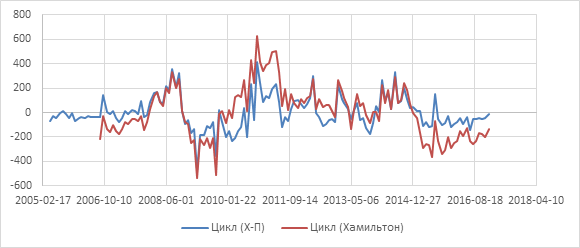
\includegraphics[width=\linewidth]{rr5.png}
		\caption{
			Циклические составляющие с шумовой компонентой для реального ВВП.
		}
		\label{fig:rr5}
	\end{figure}	
	
	\begin{figure}
		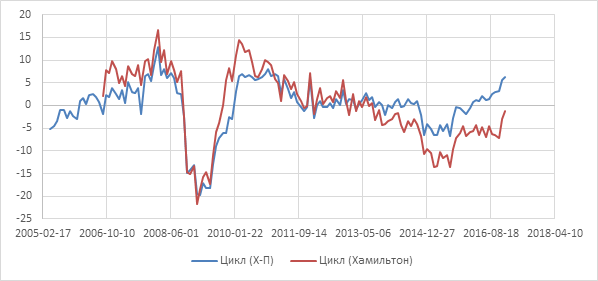
\includegraphics[width=\linewidth]{rr6.png}
		\caption{
			Циклические составляющие с шумовой компонентой для ИЭН.
		}
		\label{fig:rr6}
	\end{figure}	

	\subsection{Выделение циклов и анализ поворотных точек}
	
	Для выделения долгосрочных циклов с целью их сравнительного анализа к полученным на предыдущем этапе временным рядам  циклических составляющих с шумовыми компонентами $\hat{\nu_t}$ применяется фильтр Ходрика -- Прескотта с параметром  $\lambda=13.93$. Это позволяет удалить шумовые компоненты и получить гладкие кривые циклов для ВВП и ИЭН, представляемые на рисунках \ref{fig:rr7} и \ref{fig:rr8} соответственно. 
	
	
	\begin{figure}
		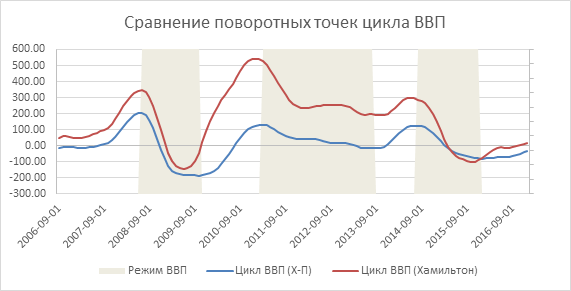
\includegraphics[width=\linewidth]{rr7.png}
		\caption{
			Сравнение поворотных точек цикла ВВП. Моменты переключения режима являются поворотными точками по Ходрику -- Прескотту. 
		}
		\label{fig:rr7}
	\end{figure}	
	
	\begin{figure}
		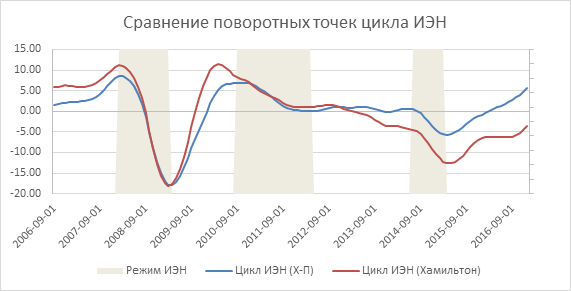
\includegraphics[width=\linewidth]{rr8.png}
		\caption{
			Сравнение поворотных точек цикла ВВП. Моменты переключения режима являются поворотными точками по Ходрику -- Прескотту.
		}
		\label{fig:rr8}
	\end{figure}	
	
	В таблице \ref{tbl:tpoints_re} приведены оценки поворотных точек циклов ВВП и ИЭН полученных с помощью фильтров Ходрика -- Прескотта и Хамильтона. 

	\begin{table}[]			
		\caption{Сравнение поворотных точек, полученные на основании разных методов фильтрации.}
			\begin{tabular}{|l|l|l|l|l|l|}
				\hline
				\multicolumn{1}{|c|}{\multirow{2}{*}{\begin{tabular}[c]{@{}c@{}}Состояние \\ экономики\end{tabular}}} & \multicolumn{1}{c|}{\multirow{2}{*}{\begin{tabular}[c]{@{}c@{}}Поворотные точки \\ реального ВВП \\ по \cite{esiMakingAlt}\end{tabular}}} & \multicolumn{2}{c|}{ВВП}                                                                                                                                      & \multicolumn{2}{c|}{ИЭН}                                                                                                                                     \\
				\multicolumn{1}{|c|}{}                                                                                & \multicolumn{1}{c|}{}                                                                                                                                      & \multicolumn{1}{c|}{\begin{tabular}[c]{@{}c@{}}Фильтр \\ Х-П\end{tabular}} & \multicolumn{1}{c|}{\begin{tabular}[c]{@{}c@{}}Фильтр\\ Хамильтона\end{tabular}} & \multicolumn{1}{c|}{\begin{tabular}[c]{@{}c@{}}Фильтр\\ Х-П\end{tabular}} & \multicolumn{1}{c|}{\begin{tabular}[c]{@{}c@{}}Фильтр\\ Хамильтона\end{tabular}} \\ \hline
				Пик                                                                                                   & 2008.06                                                                                                                                                    & 2008.06                                                                    & 2008.06                                                                          & 2008.01                                                                   & 2008.01                                                                          \\
				Дно                                                                                                   & 2009.09                                                                                                                                                    & 2009.10                                                                    & 2009.07                                                                          & 2009.03                                                                   & 2009.02                                                                          \\ \hline
				Пик                                                                                                   & 2011.03                                                                                                                                                    & 2011.03                                                                    & 2011.01                                                                          & 2010.08                                                                   & 2010.05                                                                          \\
				Дно                                                                                                   & -                                                                                                                                                          & -                                                                          & -                                                                                & 2012.04                                                                   & 2012.01                                                                          \\ \hline
				Пик                                                                                                   & -                                                                                                                                                          & -                                                                          & -                                                                                & -                                                                         & 2012.09                                                                          \\
				Дно                                                                                                   & 2013.09                                                                                                                                                    & 2013.09                                                                    & 2013.09                                                                          & -                                                                         & -                                                                                \\ \hline
				Пик                                                                                                   & 2014.07                                                                                                                                                    & 2014.07                                                                    & 2014.07                                                                          & 2014.06                                                                   & -                                                                                \\
				Дно                                                                                                   & 2016.01                                                                                                                                                    & 2016.01                                                                    & 2015.11                                                                          & 2015.03                                                                   & 2015.04                                                                          \\ \hline
			\end{tabular}
		\label{tbl:tpoints_re}	
	\end{table}
	
	Полученные в рамках настоящего исследования поворотные точки сравниваются с соответствующими значениями из \cite{esiMakingAlt}, полученные с применением фильтра Ходрика -- Прескотта. Из таблицы следует, что при использовании фильтра Ходрика -- Прескотта  в   рамках рассматриваемого интервала наблюдения с мая 2005 г. по январь 2017 г. поворотными точками являются: июнь 2008 -- пик, сентябрь 2009 -- дно, март 2011 -- пик, сентябрь 2013 -- дно, июль 2014 -- пик, январь 2016 --дно. Первая фаза экспансии (до июня 2008 г.) связана с чрезвычайно благоприятной внешней экономической конъюнктурой, а последующие (с июня 2008 г. до сентября 2009 г.) фазы замедления роста и спада связаны с воздействием на национальную экономику глобального экономического кризиса. Последующий цикл (сентябрь 2009 -- март 2011 -- сентябрь 2013) связан с «разогревом» экономики посредством инструментов экономической политики и последовавшим за этим валютным кризисом 2011 г., который привел к замедлению и спаду. Период с сентября 2013 г. по январь 2016 г. отмечен небольшим восстановлением, которое обусловлено некоторым улучшением внешней конъюнктуры и последующими затяжными фазами замедления роста и сжатия, которые были вызваны масштабными изменениями внутренней (ужесточение экономической политики) и внешней (снижение цен на сырьевые товары) среды. В то же время, не было ни одного ложного сигнала о поворотных точках. «Провал» в предсказании двух поворотных точек (сентябрь 2013 г. и июль 2014 г.) можно объяснить высокой неустойчивостью экономической конъюнктуры в этот период и, как следствие, высокой неопределенностью ожиданий экономических субъектов. Таким образом, в подобных ситуациях опережающий индикатор выступает как показатель степени неопределенности будущей экономической конъюнктуры.
	
	Оценки поворотных точек циклов для рассматриваемых временных рядов, полученные с помощью фильтров Ходрика -- Прескотта и Хамильтона, в целом достаточно близки. Тем не менее, в контексте задачи выделения экономических циклов можно указать на достаточно частое опережение моментов смены фаз циклов, получаемых с помощью фильтра Хамильтона. На такую особенность данного фильтра указывалось также в \cite{schuler_detrend}.
	
	\subsection{Выводы}
	
	Фильтры Хамильтона и Ходрика -- Прескотта  имеют  общий недостаток -- наличие априорно задаваемых параметров $h$ и $\lambda$ соответственно, от которых существенно зависят свойства получаемых трендов и циклических составляющих. Представляется, что фильтр Хамильтона более требователен к длине временных рядов.  В условиях относительно короткого времени наблюдения белорусских макроэкономических временных рядов и трудностью априорного задания параметра $h$, более предпочтительным для рассматриваемых в настоящем исследовании задач является применение фильтра Ходрика -- Прескотта. В то же время, в силу отсутствия смещения значений тренда в конечных точках и, соответственно, в остаточной составляющей, использование фильтра Хамильтона может быть предпочтительнее в  задачах прогнозирования [A4].
	

	\section{Анализ циклических изменений и оценка поворотных точек экономических циклов на основе модели с переключением состояний}
	
	\subsection{Результаты построения и применения модели MS-ARХ}
	
	Для временных рядов, скорректированных по Хамильтону, было построено несколько моделей $MS(L)-AR(p)-X(esi_{-k})$ с параметрами $L \in \{2,3\}$, $p \in \{0, ..., 3\}$, $k \in \{-1, ..., 6\}$ (см. уравнение (\ref{eq:gen-msarx})). Для сравнения моделей использовались критерии:
	
	- значимость коэфициентов модели во всех режимах,
	
	- критерий Акаике AIC,
	
	- пороговое значение частоты переключения режимов (от 2 до 10 переключений); это условие -- проверка на адекватность режимов.
	
	В результате была выбрана модель для ${GDP}$ со спецификацией $MS(2)-AR(0)-X({ESI}_{-4})$. Оцененная модель представлена уравнениями (\ref{eq:msvarx}) и (\ref{eq:msvarx_m}).
	
	{
		
		\begin{equation}
		\begin{cases}
		{GDP}_{t} = 
		\underset{[-7.827]}{-0.2042} 
		- \underset{[-3.672]}{0.3326} {ESI}_{t-4}
		+ \nu_{t} , \space \nu_{t} \sim N(0, 0.0429)
		, \quad l=0 \\
		{GDP}_{t} = 
		\underset{[17.33]}{0.4447}
		- \underset{[-4.076]}{0.2337} {ESI}_{t-4}
		+ \nu_{t} , \space \nu_{t} \sim N(0, 0.0241)
		, \quad l=1
		\end{cases}			
		\label{eq:msvarx}
		\end{equation}
		\begin{equation}
		M = 
		\begin{bmatrix}
		0.9787 & 0.0213 \\
		0.0313 & 0.9687
		\end{bmatrix}
		, \quad m_{i,j} = p[i \rightarrow j],
		\label{eq:msvarx_m}
		\end{equation}
		
	}
	
	где $m_{i,i} = p[i \rightarrow i]$ -- вероятность остаться в режиме $i$. Все коэффициенты оказались значимыми на уровне $0.05$. Графики предсказания модели (с вероятностью первого режима) представлены на рис. \ref{fig:hp-fitcompare}; остатки модели исследованы на рис. \ref{fig:hp-residcomp}.
	
	{
		\begin{figure}
			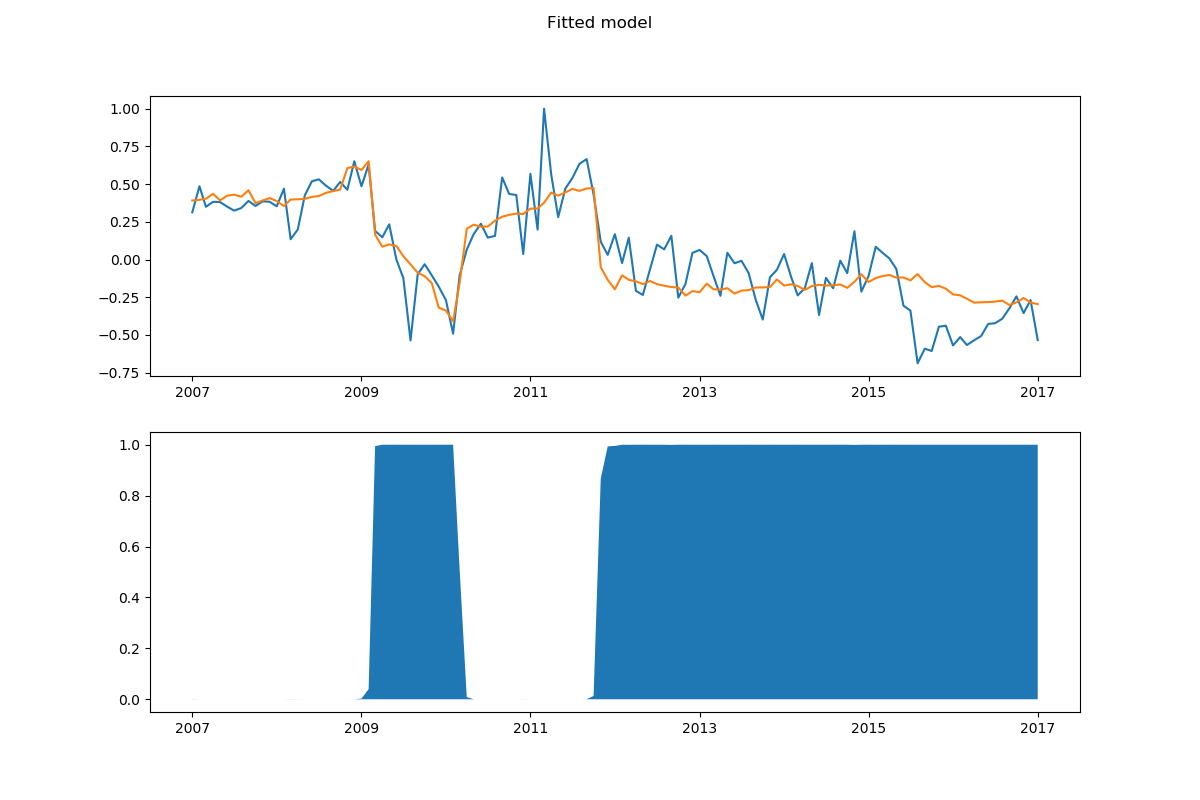
\includegraphics[width=\linewidth]{m0_fit.png}
			\caption{Предсказание модели MS(2)-ARX для ВВП по Хамильтону.}
			\label{fig:hp-fitcompare}
		\end{figure}
		\begin{figure}
			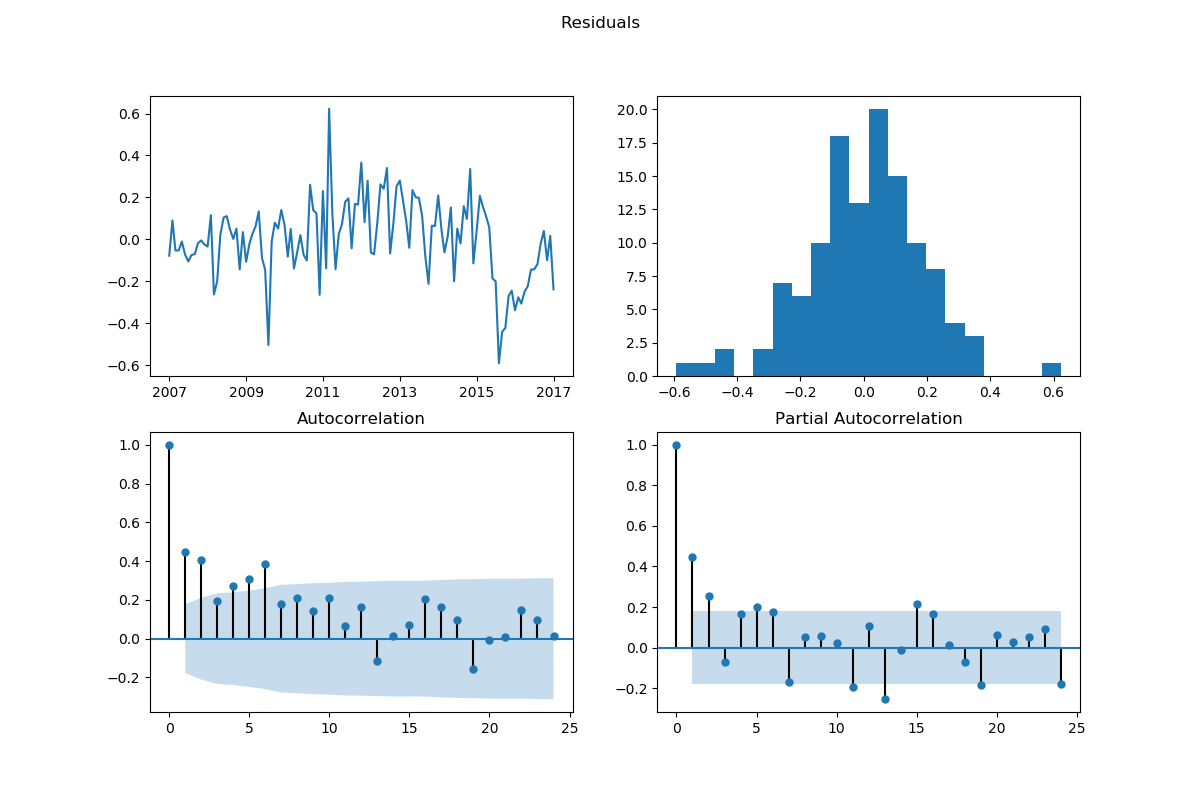
\includegraphics[width=\linewidth]{m0_resid.png}
			\caption{Анализ остатков модели для ВВП по Хамильтону.}
			\label{fig:hp-residcomp}
		\end{figure}
	}
	
	
	Аналогичным методом была построена модель для годовых темпов роста ВВП и ИЭН\footnote{от обоих рядов отнята единица для центровки}. Была выбрана модель со спецификацией $MS(2)-AR(0)-X({ESI}_{-2})$. Модель для темпов ростов исходных рядов соответствует уравнениям (\ref{eq:ms2varx}) и (\ref{eq:ms2varx_m}).
	
	Графики ВВП, модельных значений, режимов, и анализа остатков так же приведены (рис. \ref{fig:hp-fitcompare2}, \ref{fig:hp-residcompare2}).
	
	
	{
		\begin{equation}
		\begin{cases}
		{GDP}_{t} = 
		\underset{[-2.060]}{-0.007623} 
		- \underset{[-3.333]}{0.1432} {ESI}_{t-2}
		+ \nu_{t} , \space 
		, \quad l=0 \\
		{GDP}_{t} = 
		\underset{[21.78]}{0.09731}
		- \underset{[-2.785]}{0.1030} {ESI}_{t-2}
		, \quad l=1 \\
		\nu_{t} \sim N(0, 0.000786) , \quad l \in \{0, 1\}
		\end{cases},
		\label{eq:ms2varx}
		\end{equation}
		\begin{equation}
		M = 
		\begin{bmatrix}
		0.9787 & 0.0213 \\
		0.0313 & 0.9687
		\end{bmatrix}
		, \quad m_{i,j} = p[i \rightarrow j]
		.
		\label{eq:ms2varx_m}
		\end{equation}		
	}
	
	{
		\begin{figure}
			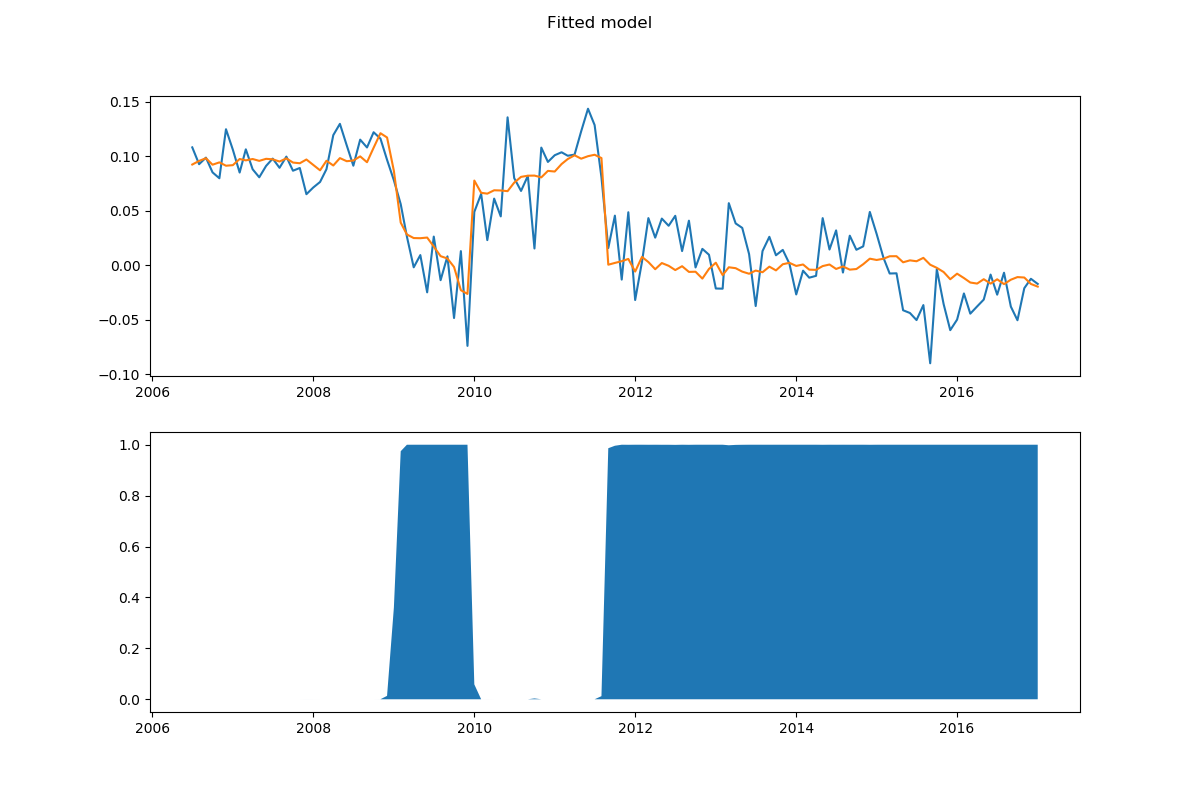
\includegraphics[width=\linewidth]{t2_fit.png}
			\caption{Предсказание модели MS(2)-ARX для темпов роста ВВП.}
			\label{fig:hp-fitcompare2}
		\end{figure}
		\begin{figure}
			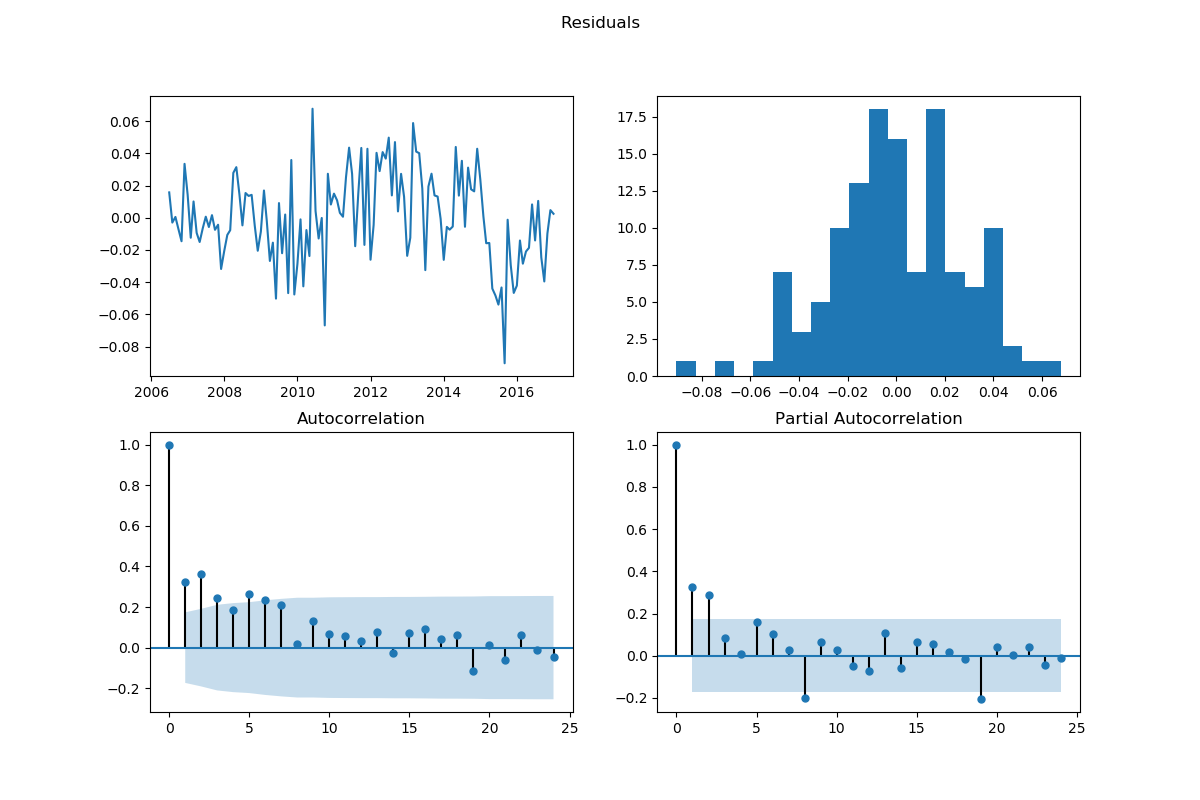
\includegraphics[width=\linewidth]{t2_resid.png}
			\caption{Анализ остатков для модели темпов роста ВВП.}
			\label{fig:hp-residcompare2}
		\end{figure}
	}
	
	% TODO: Compare models with 2 and 4 lags - at least briefly
	
	Обе модели имеют похожие результаты и свойства, несмотря на расхождение по оптимальному опережению (2 и 4). Можно предположить, что фильтр Хамильтона также может являтся приемлимым преобразованием для моделирования, однако требуются дальнейшие исследования на различных рядах.
	
	
	\subsection{Сравнительный анализ поворотных точек на основе фильтров и модели MS-ARХ}
	
	
	В табл. \ref{tbl:tpoints} приведены оценки поворотных точек разными методами. В качестве <<истинных>> значений рассматриваются экспертные оценки. Как видно, лучше всего совпадают точки, полученные в ходе двойной фильтрации (конкретно, для одной точки предсказание опаздывает на 1 месяц). Однако, точки полученные по Хамильтону (после сглаживания) отличаются не более чем на 2 месяца, причем всегда с опережением.
	
	На основании приведенных в графиках и таблице результатов можно подтвердить применимость алгоритма Хамильтона для выделения циклов. Поворотные точки циклов ВВП и ИЭН, полученные на основе данного алгоритма, либо совпадают с экспертными оценками, либо отличаются на 1--2 месяца в сторону опережения.
	
	Точки переключения режимов моделей--подклассов MS-VARX для различных рядов сильнее отличаются от истинных поворотных точек. В сравнении с другими моделями, MS-ARX для рядов, скорректированных по Хамильтону более точно предсказала первые две точки, а также третий пик, но <<пропустила>> период 2011--2013 года. Есть предположение, что моделирование с помощью MS-VARX позволит этот период описать точнее. В заключающей части этой работы производится разработка библиотеки, упрощающая создание такой модели.
	
	
	
	\begin{table}[]
	\caption{Сравнение поворотных точек, полученные разными методами.}		
	\begin{tabular}{|l|cccc|}
		\hline
		\textbf{Метод}                                                                           & \textbf{пик 1} & \textbf{дно 1}                      & \textbf{пик 2}                               & \textbf{дно 2}                             \\ \hline
		Экспертные оценки                                                                        & 2008.06        & \multicolumn{1}{c|}{2009.09}       & 2011.03                                      & 2013.09                                    \\
		Двойной HP filter                                                                        & 2008.06        & \multicolumn{1}{c|}{2009.10}        & 2011.03                                      & 2013.09                                    \\
		X13 + Hamilton (сглаж.)                                                                  & 2008.06        & \multicolumn{1}{c|}{2009.07}        & 2011.01                                      & 2013.09                                    \\ \hline
		\begin{tabular}[c]{@{}l@{}}MS-VAR для\\ индикаторов доверия\end{tabular}                 & 2008.10        & \multicolumn{1}{c|}{2010.02}        & 2011.03                                      & 2012.06                                    \\
		\begin{tabular}[c]{@{}l@{}}MS-ARX для темпов\\ роста ВВП (экзогенная -- ИЭН)\end{tabular} & 2009.01        & \multicolumn{1}{c|}{2010.01}        & 2011.09                                      & -                                          \\
		\begin{tabular}[c]{@{}l@{}}MS-ARX для Hamilton\\ ВВП (экзогенная -- ИЭН)\end{tabular}     & 2009.01        & \multicolumn{1}{c|}{2009.11}        & 2011.09                                      & -                                          \\ \hline
		\textbf{Метод}                                                                           & \textbf{пик 3} & \multicolumn{1}{c|}{\textbf{дно 3}} & \multicolumn{2}{c|}{\textbf{Замечания}}                                                   \\ \hline
		Экспертные оценки                                                                        & 2014.07        & \multicolumn{1}{c|}{2016.01}        & \multicolumn{2}{c|}{\begin{tabular}[c]{@{}c@{}}Официальные \\ оценки\end{tabular}}        \\
		Двойной HP filter                                                                        & 2014.07        & \multicolumn{1}{c|}{2016.01}        & \multicolumn{2}{c|}{\begin{tabular}[c]{@{}c@{}}Методика совпадает\\ с офиц.\end{tabular}} \\
		X13 + Hamilton (сглаж.)                                                                  & 2014.06        & \multicolumn{1}{c|}{2015.11}        & \multicolumn{2}{c|}{}                                                                     \\ \hline
		\begin{tabular}[c]{@{}l@{}}MS-VAR для\\ индикаторов доверия\end{tabular}                 & 2014.11        & \multicolumn{1}{c|}{-}              & \multicolumn{2}{c|}{см. \cite{coursework_babakhin}}                                                          \\
		\begin{tabular}[c]{@{}l@{}}MS-ARX для темпов\\ роста ВВП (экзогенная -- ИЭН)\end{tabular} & -              & \multicolumn{1}{c|}{-}              & \multicolumn{2}{c|}{}                                                                     \\
		\begin{tabular}[c]{@{}l@{}}MS-ARX для Hamilton\\ ВВП (экзогенная -- ИЭН)\end{tabular}     & -              & \multicolumn{1}{c|}{-}              & \multicolumn{2}{c|}{}                                                                     \\ \hline
	\end{tabular}
	\label{tbl:tpoints}
	\end{table}
	
	
	\section{Прогностическая способность моделей}
	
	При анализе экономических показателей, часто ставится цель прогнозирования будущего состояния временных рядов. На основании этих прогнозов выбираются стратегии дальнейших действий. Исторически, для достижения этой цели использовались авторегрессионные модели; модели MS-VARX являются расширением этого класса, поэтому возникает вопрос об их прогнозной способности в сравнении с <<обычными>> методами.
	
	\subsection{Задача валидации модели}
	
	Для оценивания прогнозной способности моделей линейной регрессии часто используется процедура, которая называется <<кросс--валидация>>, в которой случайная часть тренировочного набора выбирается в качестве тестовой выборки для оценивания поведения модели на <<новых>> данных. Однако при применении для моделирования временных рядов эта процедура имеет серъезные недостатки. Во--первых, если выбрасывать данные из <<середины>> временного ряда, то становится невозможным предсказание последующих наблюдений. Во--вторых, из--за серийной корреляции оценка ошибки предсказания будет значительно ниже чем действительное значение. Так же возникает проблема с недостатком данных, если есть только одна реализация временного ряда не очень большой длины, и характеристики ряда могут меняться со временем.
	
	Воизбежание этих проблем используется процедура <<скользящей валидации>>. Алгоритм состоит в следующим (наглядный пример ниже):
	\begin{enumerate}
		\item Выбор длины валидации $L$ для временного ряда  $y_t$ длиной $T$.
		\item Для значений $l \in \{L, L-1, ..., 1\}$:
		\begin{enumerate}
			\item Оценивается модель на данных $y_1 ... y_{T-l}$
			\item Вычисляется ошибка прогноза на один шаг вперед: 
			$\hat{\varepsilon}_{T-l+1} = y_{T-l+1} - \hat{y}_{T-l+1}$
		\end{enumerate}
		\item Считается оценка метрики (часто -- среднеквадратичное или среднее абсолютное отклонение) по $\hat{\varepsilon}_{T-L+1} ... \hat{\varepsilon}_{T}$, которая в дальнейшем используется для будущих прогнозов данного ряда.
	\end{enumerate}
	
	\begin{figure}
		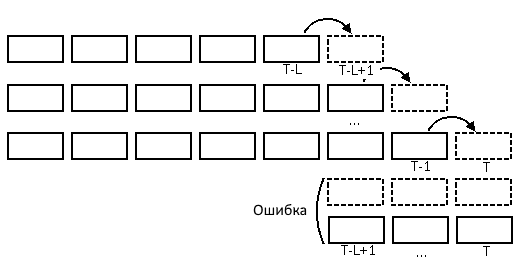
\includegraphics[width=\linewidth]{RollingValidation.png}
		\caption{Принцип скользящей валидации.}
		\label{fig:rolling_validation}
	\end{figure}
	
	Существуют и другие методологии (хороший обзор проведен в \cite{hyndCV}), но из--за небольшой длины исходных временных рядов, скользящая валидация считается самой точной.
	
	
	\subsection{Сравнение точности прогнозов моделей для ВВП}
	
	Вышеописанный подход <<скользящей валидации>> был использован для оценки точности прогноза для описанных моделей MS-ARX для годовых темпов роста ВВП (GRGDP) и для ВВП, скорректированого по Хамильтону (HamGDP). В качестве <<обычных>> методов для обоих рядов рассматривались модели модели $SARIMAX$ с автоматически подобранными порядками (алгоритм выбора описан в \cite{hynd_autoarima} и имплементирован в пакете Python \textbf{pyramid\_arima} \cite{pyramid_arima}). В таблице \ref{tbl:errors} указаны среднеабсолютые (MAE) и среднеквадратичные (RMSE) ошибки прогнозов моделей для ВВП, скорректированные по Хамильтону, и для годовых темпов роста ВВП. При сравнении необходимо учитывать, что у рядов различные масштабы. Ниже представлены графики прогнозов моделей.
	
	\begin{figure}
		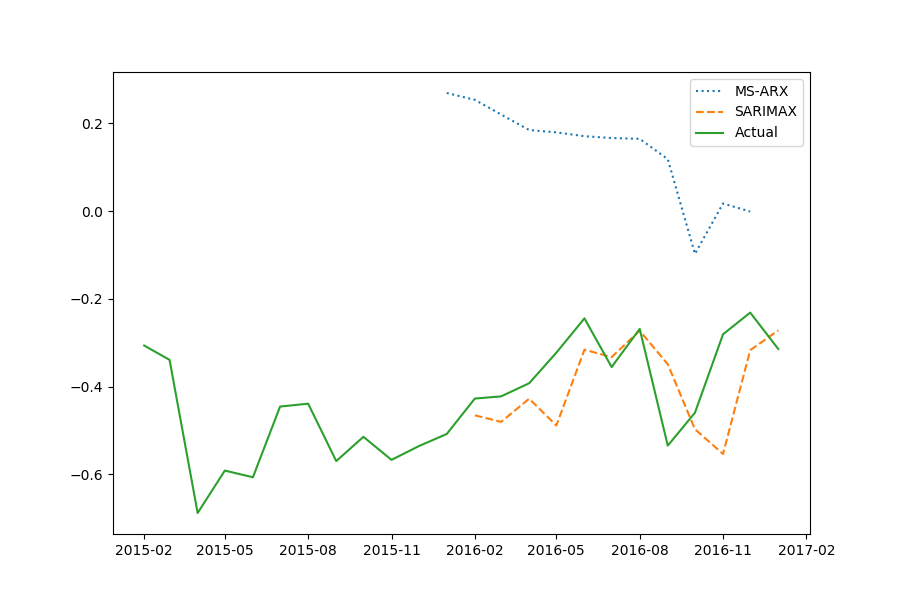
\includegraphics[width=\linewidth]{compare_ham.png}
		\caption{Сравнение скользящих прогнозов по Хамильтону.}
		\label{fig:rollcompare-ham}
	\end{figure}
	
	\begin{figure}
		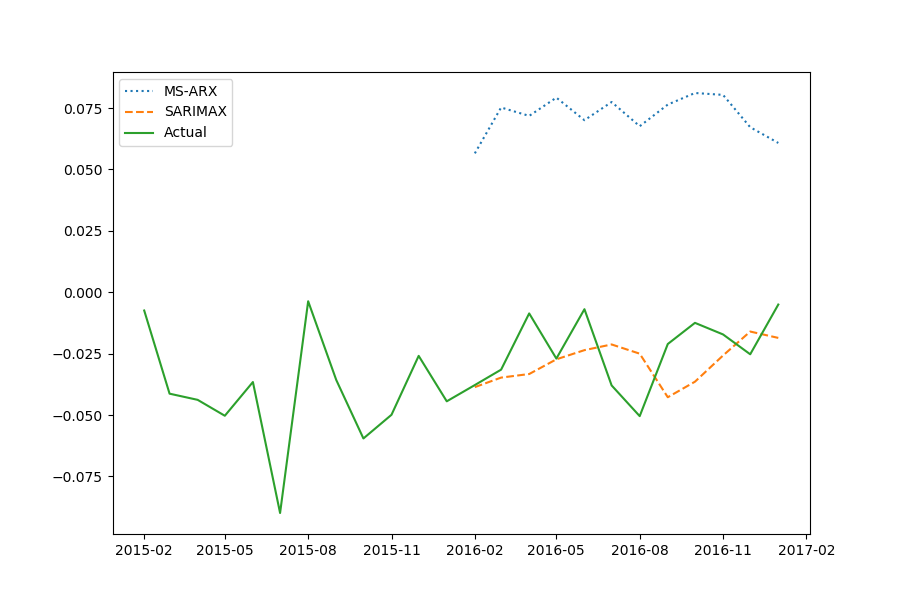
\includegraphics[width=\linewidth]{compare_gr.png}
		\caption{Сравнение скользящих прогнозов для темпов роста ВВП.}
		\label{fig:rollcompare-tr}
	\end{figure}
	
	\begin{table}[]
		\centering
		\caption{Сравнение ошибок прогонзов}
		\begin{tabular}{l|l|ll|}
			\cline{2-4}
			& Метрика & MS-ARX & SARIMAX \\ \hline
			\multicolumn{1}{|l|}{\multirow{2}{*}{ВВП по Хамильтону}}       & MAE     & 0.5646 & 0.0850  \\
			\multicolumn{1}{|l|}{}                                         & RMSE    & 0.6019 & 0.1150  \\ \hline
			\multicolumn{1}{|l|}{\multirow{2}{*}{Годовые темпы роста ВВП}} & MAE     & 0.0988 & 0.0137  \\
			\multicolumn{1}{|l|}{}                                         & RMSE    & 0.1005 & 0.0164  \\ \hline
		\end{tabular}
		\label{tbl:errors}
	\end{table}
	
	
	Как видно, модели $MS(2)-AR(0)X$ сильно уступают подобраным моделям $SARIMAX$. Можно сделать вывод, что модели переключения среднего значения не годятся для предсказывания ВВП, а только для классификации прошлых периодов (циклов) и оценивания поворотных точек.
	
	
	\chapter{Разработка библиотеки Time Series for Data Science}
	
	Одно из направлений дальнейших исследований -- векторные модели переключения состояния (MS-VARX) для отдельных секторов экономики РБ. Для оценивания параметров такой модели уже разработан EM--алгоритм \cite{malNovopMSVARX}, но он не воплощен ни в одном пакете для языков R и Python. Другое направление -- оценивание параметров при известных значениях поворотных точек, для чего также не существует пакета.
	
	Реализация алгоритмов оценивания требует больших усилий, включая работы над формализацией входных данных, проверкой предположений и выводом результатов. Для проверки корректности работы этих алгоритмов, необходимо иметь возможность сравнивать их результаты с результатами других моделей существующих пакетов. Наконец, для упрощения сравнения результатов разных моделей удобно представлять их в одинаковом формате.
	
	По этим причинам и на основания опыта работы в дисциплине <<data science>>, автором была разработана библиотека <<Time Series for Data Science>> (коротко -- \textbf{ts4ds}) на языке программирования Python. Промежуточные результаты проектирования и разработки библиотеки послужили основой выступлением на конференциях [A3, A5].
	
	\section{Краткое описание и основные задачи}
	
	\textbf{Time Series for Data Science} (сокращенно -- \textbf{ts4ds}, на русском -- <<Временные Ряды для Анализа Данных>>) -- пакет для языка программирования Python, написанный автором во время практики в компании <<ЭПАМ Системз>> (EPAM Systems). Он включает в себя средства для анализа и прогнозирования временных рядов, а также средства для разработки новых моделей. С точки зрения программного кода, он содержит базовые классы, разработанные модели, утилиты и программные тесты.
	
	При проектировании и написании пакета \textbf{ts4ds}, были поставлены следующие задачи:
	\begin{itemize}
		\item использовать методы статистического и машинного обучения для построения эконометрических моделей временных рядов;
		\item разработать обобщенное представление модели временных рядов, с целью автоматизации процессов ее построения и применения;
		\item реализовать в библиотеке процедуры построения, применения некоторых основных семейств моделей
		\item реализовать процедуры автоматизации работы с моделями (например, поиск гипер--параметров);
		\item разработать утилиты для облегчения создания новых моделей;
		\item провести тестирование компонент библиотеки (в программном и в статистическом смысле).
	\end{itemize}
	
	\section{Принципы разработки библиотеки}
	
	Для выполнения поставленных задач был необходим фундаментальный подход к проектированию и разработке библиотеки. В качестве основы брались идеи как из эконометрики, так и из дисциплины машинного обучения. Следует пояснить некоторые термины, взятые из этих дисциплин:
	
	\textbf{Модель} -- объект, описывающий (и, возможно, предсказывающий) поведение временных рядов. Математически, модель представляется параметризованными уравнениями, описывающи отношения между переменными. Эти переменные можно условно разбить на \textbf{эндогенные} (объясняемые моделью) и \textbf{экзогенные} (не объясняемые, а взятые извне и неизменяемые внутри модели).
	
	\textbf{Предиктивные модели} позволяют строить прогнозы значений временных рядов. Примерами являются авторегрессионные модели, экспоненциальное сглаживание, и рекуррентные нейросети.
	
	\textbf{Преобразования} временных рядов изменяют значения временного ряда по определенному принципу, получая при этом новый ряд. Примерами являются взятие разностей, сезонная корректировка, и методы декорреляции. (При разработке библиотеки оказалось, что преобразования удобно рассматривать как вид моделей.)
	
	\textbf{Параметры} модели -- обозначения их коэффициентов, а также значения этих коэффициентов. Иногда отдельно выделяют гиперпараметры, которые влияют на саму форму модели, но в пакете \textbf{ts4ds} такое отличие не делается.
	
	\textbf{Эстиматор} (от англ. estimator) -- алгоритм, который ищет оптимальную (по какому--то критерию) модель. Обычно этот поиск происходит в пространстве параметров, т.е. это алгоритмы оценивания параметров.
	
	Удобно рассматривать множество всевозможных моделей как функциональное пространство зависимостей между переменными. Конкретные классы моделей выделяют подмножества моделей, <<точки>> в предложенном функциональном пространстве, которые характеризуются определенной параметризацией. Например: множество линейных авторегрессионных моделей скалярной величины $AR(p)$ включают в себя подмножество авторегрессии второго порядка $AR(2)$, которое в свою очередь включает конкретную модель $AR(2)$ с коэффициентами $[-0.61, 0.22]$. В такой постановке эстиматоры можно рассматривать как алогритмы нахождения оптимальной точки (комбинации параметров) в некотором подпространстве.
	
	\section{Особенности имплементации}
	
	В библиотеке \textbf{ts4ds} каждой из вышеописанных частей соответствует отдельный класс объектов. В рамках пакета данные представляются в виде многомерного массива (numpy.ndarray) либо индексированной таблицей (pandas.Series/DataFrame) -- что является стандартом представления во всех научных библиотеках Python. Все модели -- наследники класса Model и дополнительных классов (Predictor, Transformer) с соответствующими параметрами, унаследованные от Parameters, и стандартными по интерфейсу процедурами. Эстиматоры (наследованные от Estimator) воплощают вышеописанные алгоритмы и возвращают объекты моделей вместе с параметрами.
	
	Стоит отметить, что такая организация несколько отличается от большинства традиционных библиотек. Во многих библиотеках (например, \textbf{scikit-learn}, \textbf{statsmodels}\cite{statsmodels}, и многих библиотеках языка R) процедуры оценивания параметров и процедуры выдачи предсказаний совмещены в один объект. Часто в этой структуре заодно хранят и данные. Этот подход обоснован традиционным применением: эконометрическая модель строится на одной  реализации процесса и анализируется вручную. Однако, как показывает практика, для многих промышленных применений такой традиционный подход значительно ограничивает потенциал автоматизации. 
	
	Главные недостатки традиционной организации (т.е. такой, как в \textbf{statsmodels}):
	
	\begin{itemize}
		\item неудобно сохранять модели компактно, так как нет явного понятия <<минимальных данных для воспроизведения>>;
		\item эстиматоры, которые оценивают одинакове модели (например, МНК и LASSO), должны заново воплотить процедуру предсказания; тем более, могут быть эквивалентные репрезентации, которые усложняют сравнение вычисленных параметров для одинаковых моделей;
		\item модели <<привязаны>> к данным, что делает невозможным их применение даже к данным относительно среднего размера, не говоря уже о <<больших данных>>;
		\item многие алгоритмы машинного обучения, особенно нейросети, построены с использованием отдельных структур модели, метода оценивания и данных.
	\end{itemize}
	
	Подход привязывания данных легко <<включить>> в \textbf{ts4ds}: для сохранения этой функциональности, а также и краткости записи, существует возможность <<привязать>> данные к модели через обертку BoundModel. Кроме компактной дополнительной нотации в программном коде, особых недостатков у подхода <<разделения ролей>> нет.
	
	\section{Результаты разработки}
	
	Базовые классы в библиотеке \textbf{ts4ds} -- Parameters (параметры), Model (модель), Estimator (эстиматор/алгоритм оценивания). Эти классы описывают стандартные интерфейсы для наследующих классов и, совместно с функциями в отделе <<devtools>>, освобождают от рутинной работы (например, проверки входных данных). На их основе воплощены некоторые популярные модели (и эстиматоры для них). Они служат как готовыми продуктами, которые можно использовать в работе аналитика или эконометриста, так и примерами имплементации для разработчиков собственных моделей. Все модели и эстиматоры, а также и часть утилит, автоматически проверяются программными тестами на правильность реализации конвенций интерфейса и на сходство результатов выполнения на тестовых данных.
	
	%\subsection{Базовые классы}
	
	Объект параметров (Parameters) -- набор пар ключ--значение, соответствующие именованным параметрам какой--нибудь модели, функции проверки допустимости параметров и другие вспомогательные функции.
	
	Объект модели (Model) включает в себе значение параметров и функции предсказаний (predict).
	
	Объект эстиматора (Estimator) включает в себе настройки/параметры алгоритма оценивания и реализацию этого алгоритма (fit), которая принимает набор данных и возвращает объект модели с соответствующими параметрами.
	
	%\subsection{Преобразования}
	
	Преобразования временных рядов наследованы от классов Model и Transformer. В общем случае, у преобразования существует обратное преобразование, и его форма зависит от преобразуемых данных. Поэтому удобно рассматривать преобразование как вид модели, с соответсвующими параметрами (необходимая информация для прямого и обратного преобразования) и эстиматором, который получает эти параметры. Этот подход позволяет реализовывать обратимые преобразования.
	
	В пакете на текущий момент включены следующие преобразования:
	\begin{itemize}
		\item обычные и сезонные разности, для скаляров и векторов, и обратные процедуры интегрирования;
		\item цепные трансформации, т.е. композиция преобразований.
	\end{itemize}
	
	Планируется добавить следующие преобразования:
	\begin{itemize}
		\item применение скалярных и векторных функций к каждому периоду (и, при возможности, их обратные функции);
		\item наивная сезонная декомпозиция;
		\item сезонная корректировка по процедурам X13-ARIMA-SEATS, TRAMO-SEATS;
		\item процедура выделения тренда по Хамильтону.
	\end{itemize}
	
	Ниже приведен пример работы с преобразованием взятия разности:
	
	\begin{lstlisting}[language=Python]
	from ts4ds.models.transforms.difference import Diff
	from ts4ds.models.transforms.chain import Chain_Estimator as Chain
	from ts4ds.datasets.stata_data import get_air2
	import matplotlib.pyplot as plt
	import statsmodels.api as sm
	plot_acf = sm.graphics.tsa.plot_acf
	
	y = get_air2()['lnair'] # aircraft passengers dataset
	
	# fit and transform
	dt1, y1 = Diff().fit_transform(y)
	dt12, y12 = Diff(S=12).fit_transform(y)
	dt_, y_ = Chain(Diff(), Diff(S=12)).fit_transform(y)
	
	# plotting
	fig, axs = plt.subplots(4, sharex=True)
	axs[0].plot(y)
	axs[1].plot(y1)
	axs[2].plot(y12)
	axs[3].plot(y_)
	plt.show()
	
	# Plot final ACF
	plot_acf(y_[13:], title="Final autocorrelation")
	plt.show()
	\end{lstlisting}
	
	\begin{figure}
		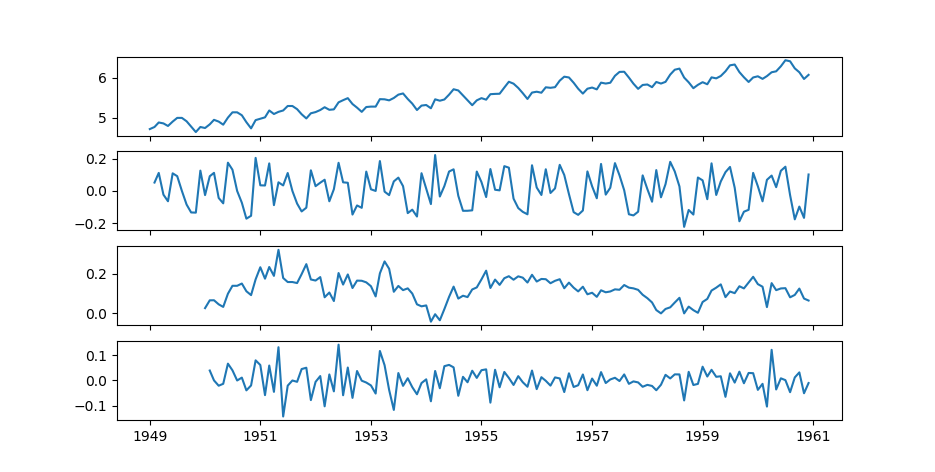
\includegraphics[width=460pt]{DiffExample.png}
		\caption{График результата выполнения (после различных трансформаций).}
		\label{fig:ts4ds-diffexample}
	\end{figure}
	\begin{figure}
		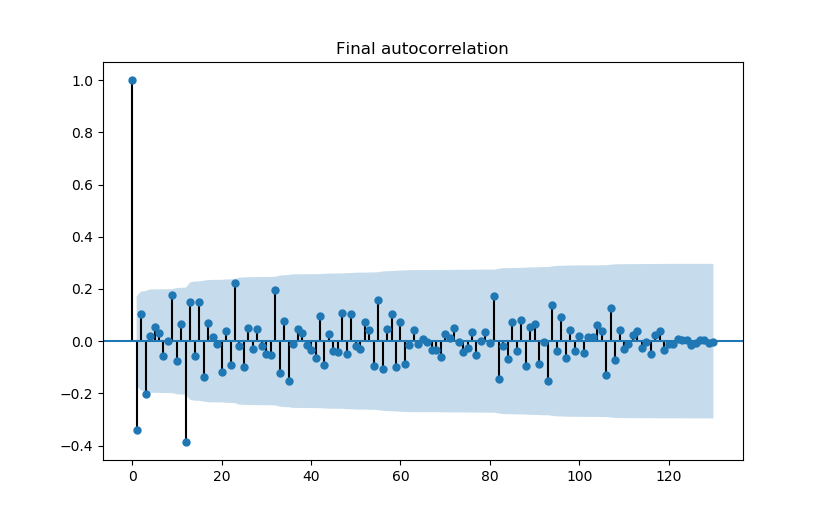
\includegraphics[width=460pt]{DiffACF.png}
		\caption{График результата выполнения (АКФ после сезонных и первых разностей).}
		\label{fig:ts4ds-diffacf}
	\end{figure}
	
	%\subsection{Предсказательные модели}
	
	В пакете \textbf{ts4ds} реализованы следующие предсказательные модели и эстиматоры для них:
	\begin{itemize}
		\item линейная регрессия;
		\item общий вид авторегрессионных моделей;
		\item модели линейной авторегрессии ARX, VARX;
		\item общая модель дискретного пространства состояний (statespace models);
		\item модели ARIMAX, SARIMAX.
		\item модели с независимыми и Марковскими переключениями состояний (семейства IS-VARX, MS-VARX).
	\end{itemize}
	
	Так же реализованы две процедуры автоматического подбора порядков для SARIMAX, так называемое <<auto\_arima>>\cite{pyramid_arima}. Пример реализации и использования модели SARIMAX описан ниже.
	
	Планируется добавить следующие модели и эстиматоры:
	\begin{itemize}
		\item модели переключения состояний (RS-models), включая MS-VARX;
		\item модели ARCH, GARCH;
		\item адаптеры для рекуррентных и сверточных нейросетей;
		\item адаптер для алгоритмов машинного обучения, изначально предназначенные для пространственных данных (например, SVM и регрессионные деревья).
	\end{itemize}
	
	
	\section{Пример: разработка модели SARIMAX}
	%\textbf{\Large Пример: разработка модели SARIMAX}
	
	Одна из самых распространенных моделей в анализе временных рядов -- модель $SARIMAX$, которая является обобщением модели $ARMA$. Полное обозначение этой модели -- $SARIMAX(p,d,q)(P,D,Q,S)$, где $S$ -- порядок сезонности, $p$ и $P$ -- порядки обычной и сезонной авторегрессии ($AR$), $d$ и $D$ -- порядки обычной и сезонной разности ($I$), $q$ и $Q$ -- порядки обычного и сезонного скользящего среднего ($MA$).
	
	Введем обозначения:
	$y_t$ -- эндогенная переменная (в момент времени $t$), 
	$x_t$ -- экзогенный вектор, 
	$\varepsilon_t$ -- вектор ошибок, 
	$L$ -- лаговый оператор, 
	$\Delta$ и $\Delta_s$ -- операторы взятия обычных и сезонных разностей, 
	$\beta$ -- вектор коэффициентов регрессии, 
	$\phi(\cdot)$, $\Phi(\cdot)$, $\theta(\cdot)$, $\Theta(\cdot)$ -- многочлены с определенными коэффициентами $AR$ и $MA$ частей соответственно.
	
	Тогда $SARIMAX(p,d,q)(P,D,Q,S)$ можно описать в форме регрессии с остатками $SARIMA$:
	
	\begin{equation}
	\begin{cases}
	y_t = \beta^{T} x_t + u_t \\
	\Phi(L) \phi(L) \Delta_s^{Q} \Delta^{q} u_t = \Theta(L) \theta(L) \varepsilon_t \\
	\varepsilon_t \sim N(0,\sigma^{2})
	\end{cases}
	\label{eq:sarimax_canonical}
	\end{equation}
	
	В случаи отсутствия экзогенных переменных, $y_t = u_t$.
	
	Для получения предсказаний в такой формулировке необходимо взять $d$ обычных и $D$ сезонных разностей, что эффективно сокращает исходный ряд на $d+SD$ периодов и усложняет задачу предсказания на эти периоды. Вместо этого, можно воспользоваться представлением в форме <<пространства состояний>> (statespace model \cite{fulton_statespace}) и предсказывать с помощью фильтра Калмана.
	
	Модель statespace описывается следующими уравнениями:
	\begin{equation}
	\begin{cases}
	\alpha_{t+1} = c + T \alpha_t + R \eta_t \\
	y_t = d + Z \alpha_t + \varepsilon_t \\
	\eta_{t} \sim N(0, Q) \\
	\varepsilon_t \sim N(0, H)
	\end{cases} 
	\label{eq:sarimax_statespace}
	\end{equation}
	
	где $y_t$ -- наблюдаемый вектор, $\alpha_t$ -- латентный (скрытый) вектор состояний, $\eta_t$ и $\varepsilon_t$ -- вектора ошибок в латентном и наблюдаемом векторе соответственно,
	$T$, $R$ и $Z$ -- матричные параметры модели, $c$ и $d$ -- вектора констант, $Q$ и $H$ -- ковариационные матрицы.
	
	Представляя в таком виде $SARIMAX$, возможно делать предсказания с помощью фильтра Калмана. Этот подход используется в пакетах \textbf{statsmodels} \cite{fulton_statespace} и \textbf{ts4ds}. Реализация фильтра Калмана в \textbf{statsmodels} очень эффективная, поэтому он используется в качестве основе для предсказаний в \textbf{ts4ds}. 
	
	На рис. \ref{fig:ts4ds-sarimax-example} показан пример использования модели SARIMAX для прогнозирования на 4 периода вперед для сезонной модели, а также ряд ошибок предсказаний (код для получения этих результатов -- в листинге).
	
	\begin{lstlisting}[language=Python]
	from ts4ds.estimators.sm_wrap.sarimax import SARIMAX_Estimator
	from ts4ds.datasets.stata_data import get_air2
	import matplotlib.pyplot as plt
	import pandas as pd
	
	y = get_air2()['lnair'] # airplane passenger dataset
	oos = pd.date_range('1961-01-01', periods=4, freq='MS') # out-of-sample
	
	# fit and predict
	model = SARIMAX_Estimator(p=1, d=1, D=1, S=12).fit(y)
	y_ins = model.predict_in_sample(y)
	y_next = model.predict(oos,y)
	y_hat = pd.concat([y_ins, y_next])
	
	# plot
	fig, axs = plt.subplots(2, sharex=True)
	h1, = axs[0].plot(y, color='0.0')
	h2, = axs[0].plot(y_hat[13:], color='red', linestyle='--')
	h4, = axs[1].plot((y_hat-y)[13:], color='0.0')
	axs[0].legend(handles=[h1,h2,h3],labels=['actual','predicted'])
	plt.show()
	\end{lstlisting}
	
	\begin{figure}
		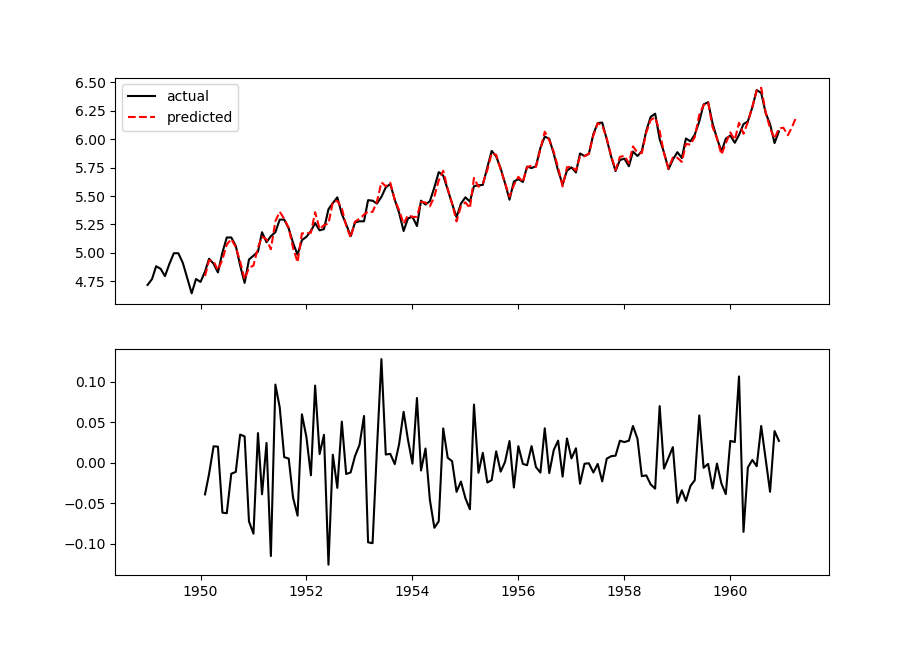
\includegraphics[width=\linewidth]{sarimax_example.png}
		\caption{Пример работы модели SARIMAX.}
		\label{fig:ts4ds-sarimax-example}
	\end{figure}
	
	%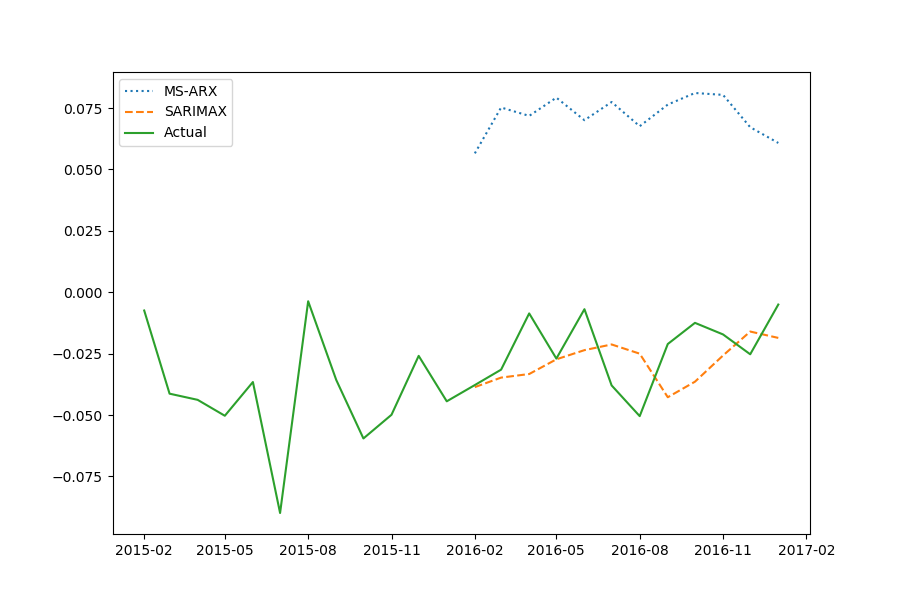
\includegraphics[width=400pt]{compare_gr.png}
	
	
	\clearpage
	
	\chapter*{}
	\bsuconclusion{
		Анализ экономических циклов и оценка моментов смены фаз циклов, называемых поворотными точками, является одной из актуальных проблем макроэкономического анализа и прогнозирования. Для проведения такого анализа используется некоторый базовый экономический индикатор, характеризующий состояние экономики, относительно которого рассчитываются показатели ее роста и спада. В качестве такого индикатора обычно используется реальный ВВП. Для прогнозирования моментов смены фаз реального ВВП традиционно применяют два подхода. 
		
		Первый подход основан на построении и применении опережающих экономических индикаторов. Индикатор считается опережающим, если поворотные точки его цикла (точки переключения фаз цикла <<спад>> и <<подъем>>) опережают поворотные точки  цикла базового экономического индикатора. В рамках данного подхода ключевыми являются две задачи: задача сезонной корректировки временных рядов базового и опережающего индикаторов и задача выделения циклической составляющей из сезонно-скорректированных временных рядов. На основе сравнения циклов для  базового и опережающего индикаторов осуществляется оценка и прогнозирование поворотных точек базового индикатора по поворотным точкам опережающего индикатора.
		
		Второй подход основан на применении эконометрических моделей с марковскими переключениями состояний. Обычно используются модели одномерной и векторной авторегрессии с марковскими переключениями состояний (MS-VAR). Для оценки поворотных точек в рамках данного подхода используются алгоритмы совместного оценивания номеров классов состояний экономики (<<спад>>/<<подъем>>) и параметров моделей.
		
		В качестве базового индикатора в работе используется месячный реальный ВВП Республики Беларусь в ценах 2014 года, а в качестве опережающего -- индекс экономических настроений (ИЭН) Республики Беларусь, построенный на основе опросных данных системы мониторинга предприятий Национального банка Республики Беларусь. Методика его построения, разработанные модельные и программные средства представлены в заключительном отчете о НИР, в рамках которой проводилось и данное исследование. Там же установлено, что поворотные точки построенного ИЭН опережают поворотные точки ВВП на 4--5 месяцев.
		
		В данной работе решалось три основные задачи:
		\begin{enumerate}
			\item сравнительный анализ двух методов выделения циклической составляющей временного ряда, включая: двойное применение фильтра Ходрика -- Прескотта (традиционный подход) и нового метода, предложенного Дж. Хамильтоном в 2017 г.  и пока не имеющего большой практики применения;
			\item построение моделей с марковскими переключениями состояний из семейства MS-VARX и сезонной модели ARIMAX, включающих в качестве экзогенной переменной опережающий индекс, и их применение для анализа экономического цикла и оценки поворотных точек;
			\item разработка библиотеки программ на языке Python для анализа временных рядов, включающая использованные в работе эконометрические модели и методы анализа, а также методы машинного обучения.
		\end{enumerate}
		
		Все решаемые задачи являются новыми и имеют практическую значимость. 
		
		Анализ циклов и их поворотных точек, полученных при решении первых двух указанных задач, а также их сравнение с экспертными оценками, полученными в рамках указанной НИР, свидетельствуют о том, что поворотные точки циклов либо совпадают, либо отличаются на 1-2 месяца для различных способов оценки. Главное несоответствие  возникает в периоде 2011-2013 гг., который характеризуется высокой неопределенностью экономической конъюнктуры.
		
		Таким образом, к числу основных результатов работы можно отнести следующие:
		
		\begin{itemize}
			\item Исследованы возможности применения методов Ходрика - Прескотта и Хамильтона для выделения циклов в экономических временных рядах;
			\item На основе этих методов оценены поворотные точки бизнес-цикла белорусской экономики и проведено их сравнене с экспертными оценками;
			\item Сделан вывод, что фильтр Ходрика - Прескотта предпочитиелен для классификации более коротких временных рядов, а фильтр Хамильтона - в задачах прогнозирования;
			\item Построены модели с переключением состояний MS-ARX для временного ряда реального ВВП Республики Беларусь, и эти модели использованы для анализа бизнес-цикла;
			\item Исследованы предиктивные возможности моделей MS-ARX и SARIMAX для реального ВВП;
			\item Спроектирована и разработана библиотека программ \textbf{ts4ds} на языке Python для анализа временных рядов;
			\item Исходный код и данные  первых двых глав работы размещены в открытом доступе на сайте {https://github.com/NowanIlfideme/PyEconModelling}, однако исходный код библиотеки на данный момент еще не опубликован.
		\end{itemize}
	}
	
	% fake chapter чтобы список лит был на одной странице
	\chapter*{}
	\addcontentsline{toc}{chapter}{Список источников}
	\markboth{Список источников}{Список источников}
	\printbibliography[title=Список источников]
	
	\chapter*{Список публкаций автора}
	\addcontentsline{toc}{chapter}{Список публкаций автора}
	\markboth{Список публкаций автора}{Список публкаций автора}
	%\printbibliography[title=Список источников]
	\begin{enumerate}[label=A\arabic*.]
		\item \textit{Макаревич А., Малюгин В.} Сравнительный анализ фильтров Ходрика -- Прескотта и Хамильтона при оценивании поворотных точек бизнес-цикла белорусской экономики / А.С. Макаревич, В.И. Малюгин // Банкаўскі веснік. -- № 8/661. Жнівень 2018. -- с. 49-56.
		
		\item \textit{Макаревич А., Малюгин В.} Построение индекса экономических настроений для Республики Беларусь / А.С. Макаревич, В.И. Малюгин // Статистические методы анализа экономики и общества: 9-я международная научно-практическая конференция студентов и аспирантов. — Национальный исследовательский университет <<Высшая школа экономики>>. 2018. — Статистические методы анализа экономики и общества: 9-я междунар. науч.-практ. конф. студентов и аспирантов.
		
		\item \textit{Makarevich A.} Automating the Process of Construction and Application of Time Series Models by Means of Machine Learning / A. Makarevich // Book of Abstracts : EURO mini-conference Logistics Analytics 2018, Minsk, 18-19 June 2018. -- p. 18.
		
		\item \textit{Макаревич А.} Сравнительный анализ оценок поворотных точек экономического цикла на основе алгоритмов Ходрика -- Прескотта и Хамильтона / А.С. Макаревич, рук. В.И. Малюгин // 74-я научная конференция студентов и аспирантов Белорусского государственного университета. — Белорусский Государственный Университет. 2017. — часть 1, с. 53-57.
		
		\item \textit{Макаревич А.} Проектирование библиотеки программ для анализа временных рядов / А.С. Макаревич, рук. В.И. Малюгин // 75-я научная конференция студентов и аспирантов Белорусского государственного университета. — Белорусский Государственный Университет. 2018. (в печати).
	\end{enumerate}
	
	% \appendix
	
	% fake chapter чтобы приложения добавлять сюда
	\chapter*{Приложения. Научные публикации автора.}
	\addcontentsline{toc}{chapter}{Приложения}
	\markboth{Приложения}{Приложения}
	
\end{document}